%% BioMed_Central_Tex_Template_v1.06
%%                                      %
%  bmc_article.tex            ver: 1.06 %
%                                       %

%%IMPORTANT: do not delete the first line of this template
%%It must be present to enable the BMC Submission system to
%%recognise this template!!

%%%%%%%%%%%%%%%%%%%%%%%%%%%%%%%%%%%%%%%%%
%%                                     %%
%%  LaTeX template for BioMed Central  %%
%%     journal article submissions     %%
%%                                     %%
%%          <8 June 2012>              %%
%%                                     %%
%%                                     %%
%%%%%%%%%%%%%%%%%%%%%%%%%%%%%%%%%%%%%%%%%


%%%%%%%%%%%%%%%%%%%%%%%%%%%%%%%%%%%%%%%%%%%%%%%%%%%%%%%%%%%%%%%%%%%%%
%%                                                                 %%
%% For instructions on how to fill out this Tex template           %%
%% document please refer to Readme.html and the instructions for   %%
%% authors page on the biomed central website                      %%
%% http://www.biomedcentral.com/info/authors/                      %%
%%                                                                 %%
%% Please do not use \input{...} to include other tex files.       %%
%% Submit your LaTeX manuscript as one .tex document.              %%
%%                                                                 %%
%% All additional figures and files should be attached             %%
%% separately and not embedded in the \TeX\ document itself.       %%
%%                                                                 %%
%% BioMed Central currently use the MikTex distribution of         %%
%% TeX for Windows) of TeX and LaTeX.  This is available from      %%
%% http://www.miktex.org                                           %%
%%                                                                 %%
%%%%%%%%%%%%%%%%%%%%%%%%%%%%%%%%%%%%%%%%%%%%%%%%%%%%%%%%%%%%%%%%%%%%%

%%% additional documentclass options:
%  [doublespacing]
%  [linenumbers]   - put the line numbers on margins

%%% loading packages, author definitions

%\documentclass[twocolumn]{bmcart}% uncomment this for twocolumn layout and comment line below
\documentclass{bmcart}

%%% Load packages
%\usepackage{amsthm,amsmath}
%\RequirePackage{natbib}
%\RequirePackage[authoryear]{natbib}% uncomment this for author-year bibliography
%\RequirePackage{hyperref}
\usepackage[utf8]{inputenc} %unicode support
%\usepackage[applemac]{inputenc} %applemac support if unicode package fails
%\usepackage[latin1]{inputenc} %UNIX support if unicode package fails
\usepackage{todonotes}
\usepackage[flushleft]{threeparttable}
\usepackage{multirow}
\usepackage{nameref}
\usepackage{amsmath}
\usepackage{hyperref}
\usepackage[table,xcdraw]{xcolor}
\usepackage{threeparttable}
\usepackage{subfig}
\usepackage[normalem]{ulem}
\usepackage{tikz}
\def\checkmark{\tikz\fill[scale=0.4](0,.35) -- (.25,0) -- (1,.7) -- (.25,.15) -- cycle;} 
\useunder{\uline}{\ul}{}


%%%%%%%%%%%%%%%%%%%%%%%%%%%%%%%%%%%%%%%%%%%%%%%%%
%%                                             %%
%%  If you wish to display your graphics for   %%
%%  your own use using includegraphic or       %%
%%  includegraphics, then comment out the      %%
%%  following two lines of code.               %%
%%  NB: These line *must* be included when     %%
%%  submitting to BMC.                         %%
%%  All figure files must be submitted as      %%
%%  separate graphics through the BMC          %%
%%  submission process, not included in the    %%
%%  submitted article.                         %%
%%                                             %%
%%%%%%%%%%%%%%%%%%%%%%%%%%%%%%%%%%%%%%%%%%%%%%%%%


% \def\includegraphic{}
% \def\includegraphics{}



%%% Put your definitions there:
\startlocaldefs
\endlocaldefs


%%% Begin ...
\begin{document}

%%% Start of article front matter
\begin{frontmatter}

\begin{fmbox}
\dochead{Research}

%%%%%%%%%%%%%%%%%%%%%%%%%%%%%%%%%%%%%%%%%%%%%%
%%                                          %%
%% Enter the title of your article here     %%
%%                                          %%
%%%%%%%%%%%%%%%%%%%%%%%%%%%%%%%%%%%%%%%%%%%%%%

% \title{Comprehensive analysis of miRNA-target interactions using Machine learning methods based on high-throughput datasets from various organisms}

\title{Comprehensive machine learning based analysis of high-throughput direct miRNA-target interactions from various organisms}

% A shorter suggestion:
% Comprehensive machine learning based analysis of high-throughput direct miRNA-target interactions.

% //maybe we can skip in the title the various organisms
%%%%%%%%%%%%%%%%%%%%%%%%%%%%%%%%%%%%%%%%%%%%%%
%%                                          %%
%% Enter the authors here                   %%
%%                                          %%
%% Specify information, if available,       %%
%% in the form:                             %%
%%   <key>={<id1>,<id2>}                    %%
%%   <key>=                                 %%
%% Comment or delete the keys which are     %%
%% not used. Repeat \author command as much %%
%% as required.                             %%
%%                                          %%
%%%%%%%%%%%%%%%%%%%%%%%%%%%%%%%%%%%%%%%%%%%%%%

\author[
   addressref={aff1},                   % id's of addresses, e.g. {aff1,aff2}
%   corref={aff1},                       % id of corresponding address, if any
%   noteref={n1},                        % id's of article notes, if any
   email={benorgi@post.bgu.ac.il}   % email address
]{\inits{GBO}\fnm{Gilad} \snm{Ben Or}}

\author[
 addressref={aff1},
%   corref={aff1},                       % id of corresponding address, if any
%   noteref={n2},                        % id's of article notes, if any
   email={vaksler@post.bgu.ac.il}
]{\inits{IVL}\fnm{Isana} \snm{Veksler-Lublinsky}}

%%%%%%%%%%%%%%%%%%%%%%%%%%%%%%%%%%%%%%%%%%%%%%
%%                                          %%
%% Enter the authors' addresses here        %%
%%                                          %%
%% Repeat \address commands as much as      %%
%% required.                                %%
%%                                          %%
%%%%%%%%%%%%%%%%%%%%%%%%%%%%%%%%%%%%%%%%%%%%%%

\address[id=aff1]{%                           % unique id
  \orgname{Department of Software and Information Systems Engineering, Ben-Gurion University of the Negev}, 
  \city{Beer Sheva},                              % city
  \cny{Israel}                                    % country
}


% \address[id=aff2]{%                           % unique id
%   \orgname{Department of Software and Information Systems Engineering, Ben-Gurion University of the Negev}, % university, etc
% %   \street{Waterloo Road},                     %
%   %\postcode{}                                % post or zip code
%   \city{Beer Sheva},                              % city
%   \cny{Israel}                                    % country
% }



% \address[id=aff2]{%
%   \orgname{Marine Ecology Department, Institute of Marine Sciences Kiel},
%   \street{D\"{u}sternbrooker Weg 20},
%   \postcode{24105}
%   \city{Kiel},
%   \cny{Germany}
% }

%%%%%%%%%%%%%%%%%%%%%%%%%%%%%%%%%%%%%%%%%%%%%%
%%                                          %%
%% Enter short notes here                   %%
%%                                          %%
%% Short notes will be after addresses      %%
%% on first page.                           %%
%%                                          %%
%%%%%%%%%%%%%%%%%%%%%%%%%%%%%%%%%%%%%%%%%%%%%%

\begin{artnotes}
%\note{Sample of title note}     % note to the article
\note[id=n1]{Equal contributor} % note, connected to author
\end{artnotes}

\end{fmbox}% comment this for two column layout

%%%%%%%%%%%%%%%%%%%%%%%%%%%%%%%%%%%%%%%%%%%%%%
%%                                          %%
%% The Abstract begins here                 %%
%%                                          %%
%% Please refer to the Instructions for     %%
%% authors on http://www.biomedcentral.com  %%
%% and include the section headings         %%
%% accordingly for your article type.       %%
%%                                          %%
%%%%%%%%%%%%%%%%%%%%%%%%%%%%%%%%%%%%%%%%%%%%%%

\begin{abstractbox}

\begin{abstract} % abstract
\parttitle{Background}
miRNAs are small non-coding RNAs that regulate gene expression post-transcriptionally. Identification of miRNA target sites on mRNAs is a fundamental step in understanding miRNA function. Several experimental high-throughput methods for identifying miRNA targets have been developed in recent years. Notably, methods that are derived from Argonaute cross‐linking and immunoprecipitation (AGO-CLIP) followed by ligation of the miRNA to its target, facilitate the identification of direct miRNA-target interactions. The limited number of such datasets promoted the use of computational prediction, in-order to further expand miRNA-target repertoires. In particular, machine learning based methods that were trained on some of these datasets were reported to achieve high accuracy performance in miRNA target prediction

% HERE SHOULD COME OUR MOTIVATION 
\parttitle{Methods and results}
In this study, we used all available high-throughput datasets from four organisms and performed comparative study of miRNA-target interactions. We have developed a processing pipeline and performed comprehensive comparative analysis. Then, we evaluated 6 machine learning methods for miRNA-target prediction, analyzed the results and examined the importance of each feature. Finally, We explored the relationship between datasets and tested the performance of inter-datasets miRNA-target prediction.
\parttitle{Conclusions}
Our work proposes an analysis method for miRNA-target interaction datasets, offers valuable insights into potential advances in target prediction methods, and shows that transferability of rules from organism to organism can be a promising method for studying the interaction of organisms without sufficient experimental data.

\parttitle{Availability and implementation} The code is freely available at \url{https://github.com/gbenor/TPVOD}
\end{abstract}

%%%%%%%%%%%%%%%%%%%%%%%%%%%%%%%%%%%%%%%%%%%%%%
%%                                          %%
%% The keywords begin here                  %%
%%                                          %%
%% Put each keyword in separate \kwd{}.     %%
%%                                          %%
%%%%%%%%%%%%%%%%%%%%%%%%%%%%%%%%%%%%%%%%%%%%%%

\begin{keyword}
\kwd{Machine learning}
\kwd{miRNA}
\kwd{Target prediction}
\kwd{CLASH}
\kwd{AGO-CLIP}
\kwd{chimeric miRNA-target interactions}
\end{keyword}

% MSC classifications codes, if any
%\begin{keyword}[class=AMS]
%\kwd[Primary ]{}
%\kwd{}
%\kwd[; secondary ]{}
%\end{keyword}

\end{abstractbox}
%
%\end{fmbox}% uncomment this for twcolumn layout

\end{frontmatter}

%%%%%%%%%%%%%%%%%%%%%%%%%%%%%%%%%%%%%%%%%%%%%%
%%                                          %%
%% The Main Body begins here                %%
%%                                          %%
%% Please refer to the instructions for     %%
%% authors on:                              %%
%% http://www.biomedcentral.com/info/authors%%
%% and include the section headings         %%
%% accordingly for your article type.       %%
%%                                          %%
%% See the Results and Discussion section   %%
%% for details on how to create sub-sections%%
%%                                          %%
%% use \cite{...} to cite references        %%
%%  \cite{koon} and                         %%
%%  \cite{oreg,khar,zvai,xjon,schn,pond}    %%
%%  \nocite{smith,marg,hunn,advi,koha,mouse}%%
%%                                          %%
%%%%%%%%%%%%%%%%%%%%%%%%%%%%%%%%%%%%%%%%%%%%%%
\section*{Introduction}
% \subsection*{miRNAs summary}
miRNAs are small non-coding RNAs that regulate gene expression post-transcriptionally. The functional mature miRNAs are generated in a multi-stage process \cite{finnegan2013microrna} and are eventually associate with Argonaute proteins to form the core of the miRNA-induced silencing complex (miRISC). miRISC uses the sequence information in the miRNA as a guide to bind complementary sequences on mRNAs, to repress  translation or degrade targeted mRNAs \cite{huntzinger2011gene}. 
miRNAs are conserved throughout evolution, and are present in the genomes of animals, plants and in some viruses \cite{kozomara2013mirbase}. MiRNAs function in diverse aspects of development and physiology and have been implicated in human disease \cite{rupaimoole2017microrna}.

\subsection*{Identification of miRNA-target interactions}
Identification of miRNA target sites on mRNAs is a fundamental step in understanding miRNA function.
Several experimental high-throughput methods for identifying miRNA targets have been developed in recent years \cite{li2019current, martinez2013microrna}.
The most straightforward approach relies on transfection of specific miRNA mimics or inhibitors into the cells followed by high-throughput analysis of mRNA expression (by microarray or high-throughput sequencing), or proteomics \cite{thomas2010desperately}. However, this approach cannot distinguish direct from indirect targets. 


Other methods that are based on crosslinking and immunoprecipitation (CLIP) use ultraviolet (UV) light to covalently conjugate protein-RNA complexes. After immunoprecipitation with a specific AGO antibody (AGO-CLIP), miRNAs, their targets and AGO protein are precipitated together for further sequencing analysis \cite{chi2009argonaute, hafner2010transcriptome, zisoulis2010comprehensive}. Though these methods greatly decrease the target search space to specific regions on mRNAs, the identity of the miRNA engaged in each interaction is unknown and has to be predicted bioinformatically \cite{wang2015design, uhl2017computational}.

Recently, several high-throughput methods, e.g., CLASH, that can capture miRNAs bound to their respective targets have been developed \cite{scheel2017global, grosswendt2014unambiguous, darnell_moore2015mirna, helwak2013mapping}. These methods are derived from Argonaute cross‐linking and immunoprecipitation (AGO-CLIP) and use an extra step to covalently ligate the miRNA and the target RNA. Subsequent cloning and sequencing of isolated RNAs capture short chimeric miRNA‐target reads which facilitates the identification of direct miRNA‐target interactions. An additional method iCLIP \cite{broughton2016pairing} that was applied to \textit{C. elegans} reported a recovery of chimeric sequences without employing the ligation step. Furthermore, reanalysis of published mammalian AGO-CLIP data recovered additional  miRNA-target chimeric interactions in libraries where no ligase was added \cite{grosswendt2014unambiguous}. 
The analysis of these interactions revealed that many of them consist of non-canonical seed binding patterns and involve nucleotides outside the seed regions. Despite the great contribution that these experimental methods can bring to the field, their application is technically challenging and so far, datasets were generated for only a small number of model organisms (Table \ref{tbl:dataset_description}).

\subsubsection*{Computational miRNA-target prediction}
The limited number of experimentally identified miRNA-target interactions promoted the use of computational prediction in-order to expand miRNA-target repertoires. Nevertheless, computational identification is also very challenging, since miRNAs are short and engage only a limited sequence complementarity to their targets. 
Over the past 15 years, many computational tools were developed for this task. The first generation of tools was based on very general rules of thumb, e.g., canonical seed pairing, miRNA-target duplex energy, conservation of the target site and accessibility \cite{kruger2006rnahybrid, enright2003microrna, lewis2005conserved, kertesz2007role}. These tools suffer from high False Positive and False Negative prediction rates \cite{pinzon2017microrna, oliveira2017combining, fridrich2019too, min2010got}, due to very general rules and insufficient knowledge about seedless interactions and base pairing patterns in the non-seed region. In addition, the outputs of these tools show only partial overlap, making it difficult to choose candidates for further experimental validation or more global downstream analysis.

The availability of new datasets of high-throughput, direct miRNA-target interactions (e.g., \cite{scheel2017global, grosswendt2014unambiguous, darnell_moore2015mirna, helwak2013mapping}), led to the development of new machine-learning (ML) based methods for miRNA target prediction \cite{lu2016learning, ding2016tarpmir, pla2018miraw, wen2018deepmirtar, cheng2015mirtdl, menor2014mirmark}. These methods were designed to capture also non-canonical sites and pairing beyond the seed region, by introducing tens to hundreds different features (representing e.g., sequence, structure, conservation, context), and were reported to achieve significant improvement in overall predictive performance than the previous tools. Differences in several aspects can be observed among ML-based methods, including the ML approach and the features used, the choice of datasets for training and testing, inclusion or exclusion of non-canonical interaction from the training/testing set, and the approach of generating negative data. We provide a summary of some of these methods, focusing on these aspects, in \nameref{add:figs_tbls}, Table S1. 

Briefly, the methods chimiRic \cite{lu2016learning} and miRTarget \cite{wang2016improving,liu2019prediction} use support vector machine (SVM) for classifying miRNA-target interactions. TarPmiR \cite{ding2016tarpmir} is a random-forest (RF) based approach that provides a probability that a candidate target site is a true target site. DeepMirTar \cite{wen2018deepmirtar}, miRAW \cite{pla2018miraw}  and mirLSTM \cite{paker2019mirlstm} apply deep learning approaches that are based on on stacked de-noising auto-encoder (SdA), deep artificial neural networks (ANN) and long short term memory (LSTM), respectively.  

Most of the above-mentioned studies trained and tested their models on CLASH based dataset from human \cite{helwak2013mapping}, and then used independent datasets for additional testing. The main training/testing dataset of TarPmir \cite{ding2016tarpmir}, was composed primarily from human CLASH dataset. DeepMirTar \cite{wen2018deepmirtar} and mirLSTM \cite{paker2019mirlstm} included also additional small number of interactions retrieved from miRecords \cite{xiao2009mirecords}. Other studies complemented their datasets by seed-containing sites from AGO-CLIP data (e.g., chimiRic \cite{lu2016learning}, miRAW \cite{pla2018miraw}) or chimeras generated by endogenous ligation in human AGO-CLIP experiments (e.g., miRTarget \cite{wang2016improving}). Some studies intersected the CLASH data with other resources to retain only interactions with functional evidence (e.g., miRAW \cite{pla2018miraw} and  miRTarget v4 \cite{liu2019prediction}).

For independent testing, the above methods used various datasets, not necessarily derived from ligation-based experiments. 
DeepMirTar \cite{wen2018deepmirtar} was tested on human PAR-CLIP dataset, TarPmir \cite{ding2016tarpmir} was tested on two PAR-CLIP human datasets and a HITS-CLIP dataset from mouse, while chimiRic \cite{lu2016learning} model was tested on chimeric interactions from  \textit{C. elegans} \cite{grosswendt2014unambiguous} and mouse \cite{darnell_moore2015mirna}. Additional evaluation with microarray datasets following miRNA transfections or miRNA knockdowns, was performed by miRAW \cite{pla2018miraw}  and miRTarget (\cite{wang2016improving,liu2019prediction}, respectively. 

\subsection*{Motivation to our study}
Based on the survey above it is evident that current ML-based tools learn interaction rules from experimental datasets which are limited to only a few model organisms. Nevertheless, there is a need to apply these tools on other organisms as well, where experimental data is not available.
However, the extent to which miRNA-target interaction rules are transferable from one organism to another, was not thoroughly studied.

Though some of the ML methods mentioned above examined the possibility to predict interactions in organisms different from the organism they were trained on, in all cases the training was performed on human datasets, and was applied on a few other organisms. The ability to do the predictions in the opposite direction, or between organisms other than human were not tested.Moreover, it was not been previously assessed how different characteristics of the training and the testing sets affect the performance of miRNA-target prediction models.  

Furthermore, we hypothesize that the process of miRNA targeting, which is governed by the miRISC complex, underwent at least some changes during evolution, affecting the features that characterize the interactions in different organisms. However, we also hypothesize that there is a set of features that has been fixed during evolution. The availability of high-throughput miRNA-target interactions data across several organisms provides us with the opportunity to address these hypotheses. 

\subsection*{Summary}
In this paper we use available high-throughput datasets from four organisms and perform comparative study of miRNA-target interactions. Eight datasets from various organisms, tissues and experimental protocols have been evaluated. We have developed a processing pipeline to transform these datasets into a standard format that enables comprehensive comparative analysis. We provide a detailed overview of the datasets, focusing on their sizes, seed families composition and interaction patterns, while highlighting their resemblance and dissimilarity. For each dataset, we trained and tested 6 different machine learning classifiers for the prediction of miRNA-target interactions, and evaluated the importance of the features we used.
We then explored the relationship between datasets by measuring the divergence of their seed sequences, and by evaluating the performance of inter-datasets classification. Our results indicate that the transferability of miRNA-targeting rules between different organisms depends on several factors, including composition of seed families and evolutionary distance. Our study provides important insights for future developments of target prediction tools that could be applied on organisms without sufficient experimental data.


%%%%%%%%%%%%%%%%%%%%%%%%%%%%%%%%%%%%%%%%%%%%%%%%%%%
% Results
%%%%%%%%%%%%%%%%%%%%%%%%%%%%%%%%%%%%%%%%%%%%%%%%%%%%

\clearpage
\section*{Results}
\subsection*{Dataset processing}
Eight miRNA-target chimera datasets were generated so far for human, mouse, the nematode \textit{Caenorhabditis elegans (C.elegans)} and the cattle \textit{Bos taurus}.
Table \ref{tbl:dataset_description} provides the details for each dataset, including the cell type or developmental stage that was examined and the experimental protocol that was used. Five of the datasets were generated by methods that use AGO-CLIP with an extra step to covalently ligate the miRNA and the target RNA (\textit{ca1}, \textit{ce1}, \textit{h1},  \textit{h3}, \textit{m2}). Additional \textit{C.elegans} dataset (\textit{ce2}) contains chimeras recovered from an iCLIP experiment that did not apply an additional ligation step. Two mammalian datasets (\textit{h2}, \textit{m1}) were generated by reanalysis of published mammalian AGO-CLIP data which also recovered miRNA-chimeras in libraries where no ligase was added \cite{grosswendt2014unambiguous}. The latter two datasets contain chimeras from several independent experiments (thus denoted as a "mix").

A multi-step processing pipeline was applied to (1) retrieve all the needed information about the interactions, (2) filter out non 3'UTR interactions, (3) generate miRNA-target duplexes, and (4) keep only the interactions with canonical or non-canonical seeds. The 3'UTR interactions represent 10\%-47\% of all interactions in the datasets and interactions with canonical or non-canonical seed pairing constitute 53\%-82\% of them. The pipeline produced final datasets with variable sizes: four small datasets (500-1200), two large datasets (2000-5000) and two massive datasets ($\sim$18,000 each). The numbers of interactions passing the filters are shown in Table \ref{tal:pipeline_summary}.

The final datasets generated by the pipeline are later used as input for machine learning tasks. Therefore, we complemented the datasets with synthetically-generated negative interactions as described in methods. We extracted 490 features from each interaction, representing proprieties of the interaction duplex and interaction site and its flanking region within the 3'UTR (see methods: \nameref{methods_features}).

\begin{table}[h!]
\caption{Datasets information}
\label{tbl:dataset_description}
% \begin{tabular}{ | l | l | l | l | l | }
\begin{tabular}{|l|p{6cm}|p{4cm}|l|}
	\hline
	\textbf{Name} & \textbf{Cell/ Developmental stage} & \textbf{Experimental Method} & \textbf{Reference} &
	\hline
	
% 	cattle\_MDBK & 
    ca1 &
	Madin-Darby bovine kidney (MDBK) & 
	CLEAR-CLIP                        
	& \cite{scheel2017global} & 
	\hline
	
% 	celegans\_L3 & 
    ce1 &
	L3 staged & 
	Modified iPAR-CLIP & 
	\cite{grosswendt2014unambiguous} & 
	\hline

% 	celegans\_L4 & 
    ce2 &
	mid-L4 WT (N2)  & 
	ALG-1 iCLIP endogenous ligation & 
	\cite{broughton2016pairing} &
	\hline

% 	human\_HEK293 & 
    h1 &
	Human embryonic kidney293 cells (HEK293) & 
	CLASH  & 
	\cite{helwak2013mapping} &
	\hline
	
% 	human\_mix & 
    h2 &
	A mix of 6 datasets, each interaction is annotated with the experiment & 
	endogenous ligation &  
	\cite{grosswendt2014unambiguous} &
	\hline
	
% 	human\_huh7.5 & 
    h3 &
	human hepatoma cells (Huh-7.5) & 
	CLEAR-CLIP & 
	\cite{darnell_moore2015mirna} &
	\hline
	
% 	mouse\_mix & 
    m1 &
	A mix of 3 datasets, each interaction is annotated with the experiment & 
	endogenous ligation & 
	\cite{grosswendt2014unambiguous} &
	\hline
	
% 	mouse\_ATCC & 
    m2 &
	N2A mouse neuroblastoma (ATCC) & 
	CLEAR-CLIP & 
	\cite{darnell_moore2015mirna} &
	\hline
\end{tabular}
\end{table}



\begin{table}[h!]
\caption{Summary of data processing pipeline}
      \label{tal:pipeline_summary}
                 \begin{threeparttable}
      \begin{tabular}{|l|l|l|l|l|l|l|l|l|}

\hline
\textbf{Dataset}                                                                                   & \textbf{ca1}     & \textbf{ce1}   & \textbf{ce2}   & \textbf{h1}     & \textbf{h2}     & \textbf{h3}     & \textbf{m1}    & \textbf{m2}      \\ \hline
No. of interactions \tnote{a}                                                                         & 296,297 & 3,627 & 4,920 & 18,514 & 10,567 & 32,712 & 1,986 & 130,094 \\ \hline
No. of interactions in 3'UTR                                                                 & 30,534  & 1,704 & 1,206 & 8,507  & 2,039  & 4,634  & 902   & 33,100  \\ \hline
\textbf{\begin{tabular}[c]{@{}l@{}}Final dataset\\ (canonical \& non-canonical\\ interactions)\end{tabular}} & \textbf{18,204} & \textbf{1,176} & \textbf{992} & \textbf{5,137} & \textbf{1,150} & \textbf{2,846} & \textbf{537} & \textbf{17,574} \\ \hline
\end{tabular}
\begin{tablenotes}
            \item[a] As provided by the original publicationץ
        \end{tablenotes}
     \end{threeparttable}
\end{table}

\subsection*{Dataset characteristics}
We assessed the quality and the characteristics of the datasets by statistical analyses and tests and visualized the results. Since the negative interactions are synthetically-generated, the analyses described in the following subsections refer to positive interactions only.

\subsubsection*{miRNA distribution}
We counted the appearance of miRNA sequences and seed families (nt2-7) and generated a distribution function for each dataset (Table \ref{tbl:mircontribution}). Our analysis indicates that the datasets are not uniformly distributed in terms of miRNA appearances (Figure \ref{fig:datasetplot}). Furthermore, 90\% of the interactions are dominated by a small subset of miRNA sequences (25-50\%) or miRNA seed families (18-37\%).

\begin{table}[h!]
\caption{Composition of miRNA sequences and miRNA seed families within datasets}
\label{tbl:mircontribution}
\begin{tabular}{|l|l|l|l|l|l|l|l|l|}
\hline
\textbf{Dataset}          & \textbf{ca1}                                                  & \textbf{ce1}                                                  & \textbf{ce2}                                                  & \textbf{h1}                                                   & \textbf{h2}                                                   & \textbf{h3}                                                   & \textbf{m1}                                                   & \textbf{m2}                                                    \\ \hline
\textbf{No. of interactions}   & 18,204  & 1,176 & 992   & 5,137  & 1,150  & 2,846  & 537   & 17,574                                                 \\ \hline
\textbf{No. of miRNA sequences}      & 165                                                  & 68                                                   & 56                                                   & 287                                                  & 140                                                  & 203                                                  & 98                                                   & 417                                                   \\ \hline
\textbf{90\% point [miRNA sequences]} & \begin{tabular}[c]{@{}l@{}}49 \\ (29\%)\end{tabular} & \begin{tabular}[c]{@{}l@{}}26 \\ (38\%)\end{tabular} & \begin{tabular}[c]{@{}l@{}}24 \\ (42\%)\end{tabular} & \begin{tabular}[c]{@{}l@{}}99 \\ (34\%)\end{tabular} & \begin{tabular}[c]{@{}l@{}}58 \\ (41\%)\end{tabular} & \begin{tabular}[c]{@{}l@{}}68 \\ (33\%)\end{tabular} & \begin{tabular}[c]{@{}l@{}}49 \\ (50\%)\end{tabular} & \begin{tabular}[c]{@{}l@{}}111 \\ (26\%)\end{tabular} \\  \hline
\textbf{No. of seed families}      & 119                                                  & 46                                                   & 35                                                   & 254                                                  & 133                                                  & 191                                                  & 88                                                   & 343                                                   \\ \hline
\textbf{90\% point [seed families]}  & \begin{tabular}[c]{@{}l@{}}21 \\ (18\%)\end{tabular} & \begin{tabular}[c]{@{}l@{}}14 \\ (30\%)\end{tabular} & \begin{tabular}[c]{@{}l@{}}13 \\ (37\%)\end{tabular} & \begin{tabular}[c]{@{}l@{}}62 \\ (24\%)\end{tabular} & \begin{tabular}[c]{@{}l@{}}35 \\ (26\%)\end{tabular} & \begin{tabular}[c]{@{}l@{}}42 \\ (22\%)\end{tabular} & \begin{tabular}[c]{@{}l@{}}30 \\ (34\%)\end{tabular} & \begin{tabular}[c]{@{}l@{}}63 \\ (18\%)\end{tabular}  \\ \hline
\end{tabular}
\end{table}


\begin{figure}[h!]
  \caption{\csentence{Cumulative sum of miRNA sequence appearances in the examined datasets.} Each curve corresponds to the cumulative sum of one of the datasets, where the bold points indicate the minimum number of unique miRNA sequences needed to represent 90\% of the interactions within a dataset. The height of a curve represents the size of the dataset, and the width of a curve represents the number of unique miRNA sequences that comprise the dataset.}
      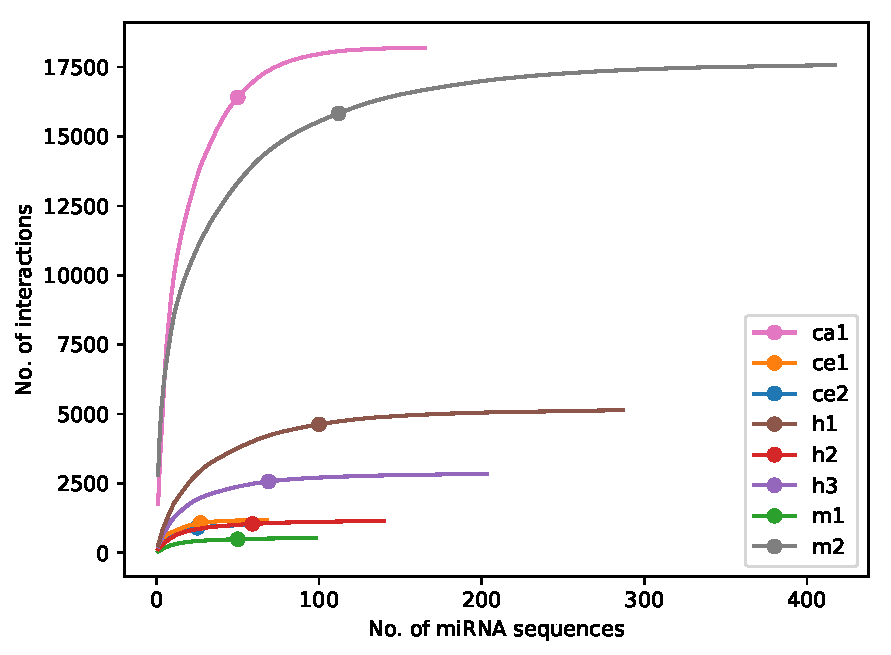
\includegraphics[width = 1\textwidth]{Results/mirna_dist.pdf}
      \label{fig:datasetplot}
      \end{figure}


\subsubsection*{Seed types and base-pairing density}
We classified the interactions (i.e., the corresponding duplexes formed by the miRNA and the target site) based on two parameters: seed type (canonical or non-canonical, see methods) and base-pairing density (number of base-pairs (bp) within the duplex: low with less than 11bp, medium with 11-16bp and high with more than 16bp). We defined 6 groups based on  combinations of seed type and base-pairing density and assigned each interaction to the appropriate group (Figure \ref{fig:seed_type_pos}). As can been seen in the figure, the datasets are rich and diverse, and include all the combinations of seed type and base-pairing density.
% In particular, we would like to enlight 2 points: 
Nevertheless, two observations stand out: 
(1) In terms of seed type, majority of the interactions are non-canonical (48-70\%); and (2) for both groups of seed types,  majority of the interactions have medium and high base-pairing density, while the low base-pairing density interactions comprise only a small portion of the datasets. Similar analysis for the negative interactions is shown in \nameref{add:figs_tbls}, Figure S1.

\begin{figure}[h!]
  \caption{\csentence{Types of positive miRNA-target duplexes.} The percentage of miRNA-target duplexes shown in 6 groups according to the seed type (canonical and non-canonical) and to the base-pairing density (low: less than 11bp, medium: 11-16bp and high: more than 16bp).}
    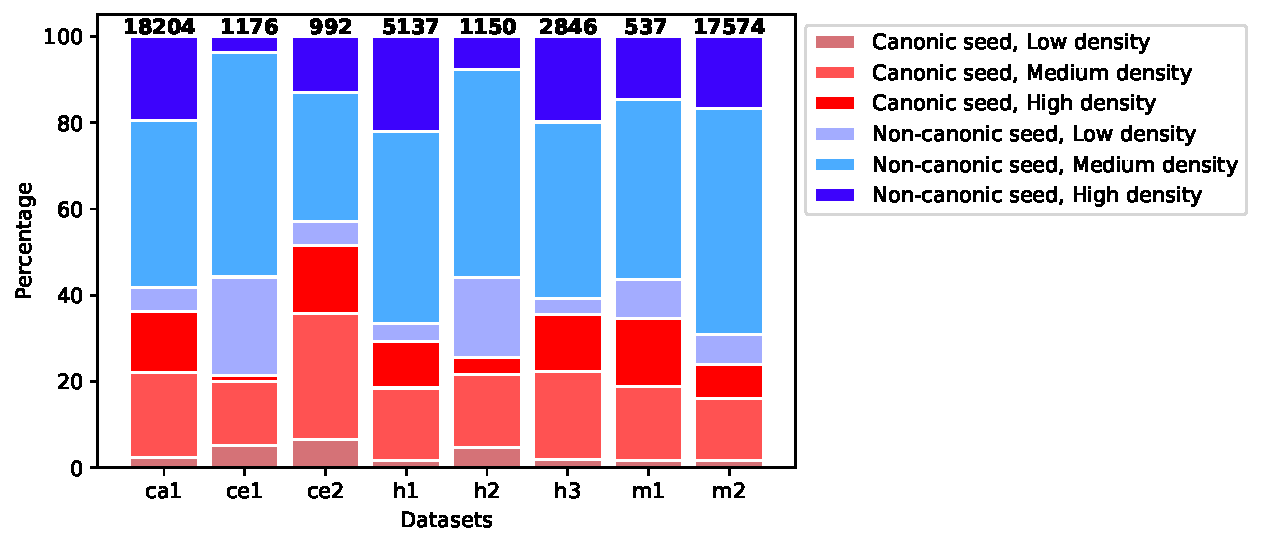
\includegraphics[width = 1\textwidth]{Results/seed_type_positive2.pdf}
      \label{fig:seed_type_pos}
      \end{figure}


\subsubsection*{Dataset visualization}
Visualization is an important step in the analysis of high-throughput biological data and can assist in revealing hidden phenomena. However, visualization is challenging when the data is represented by a large number of features. Dimensionality reduction algorithm enables the representation of the data in 2-dimension scatter plot and facilitates the inspection of the data by eye. MiRNA-target interactions in our study are represented by 490 features (see methods). To visualize the datasets in 2D, we performed a dimensional reduction using the PCA technique (Figure \ref{fig:feature_pca}). The 2D representation explains 67\% of the variance, where percentage of variance explained by the x and the y axes are 52 and 15, respectively. 

Figure \ref{fig:feature_pca} reiterates the fact that there are big differences in the sizes of the datasets, reflected in the density of the graphs. For example, the size of the human dataset \textit{h1} is more than twice the size of the datasets \textit{h2} and \textit{h3}, and indeed, its graph is denser. In addition, there are notable differences in the 2-dimensional space spanned by each dataset: while the datasets of human, cattle and mouse are spread in the whole area, \textit{C.elegans} datasets are concentrated in a narrower part of the area. Moreover, a comparison of datasets coming from the same organism, shows that datasets composed of endogenous ligation chimeras from a mixture of experiments (\textit{h2}, \textit{m1}), have a lower spread than datasets originating from a protocol with ligation step (\textit{h1},\textit{h3},\textit{m2}).

%%%% Problems with printing this format
% \begin{figure}[h!]
%   \caption{\csentence{Datasets presented in 2D.} Each point represents a single interaction after a dimensional reduction of its feature space using PCA. X and Y axes are the first and the second component of the PCA respectively.}
%       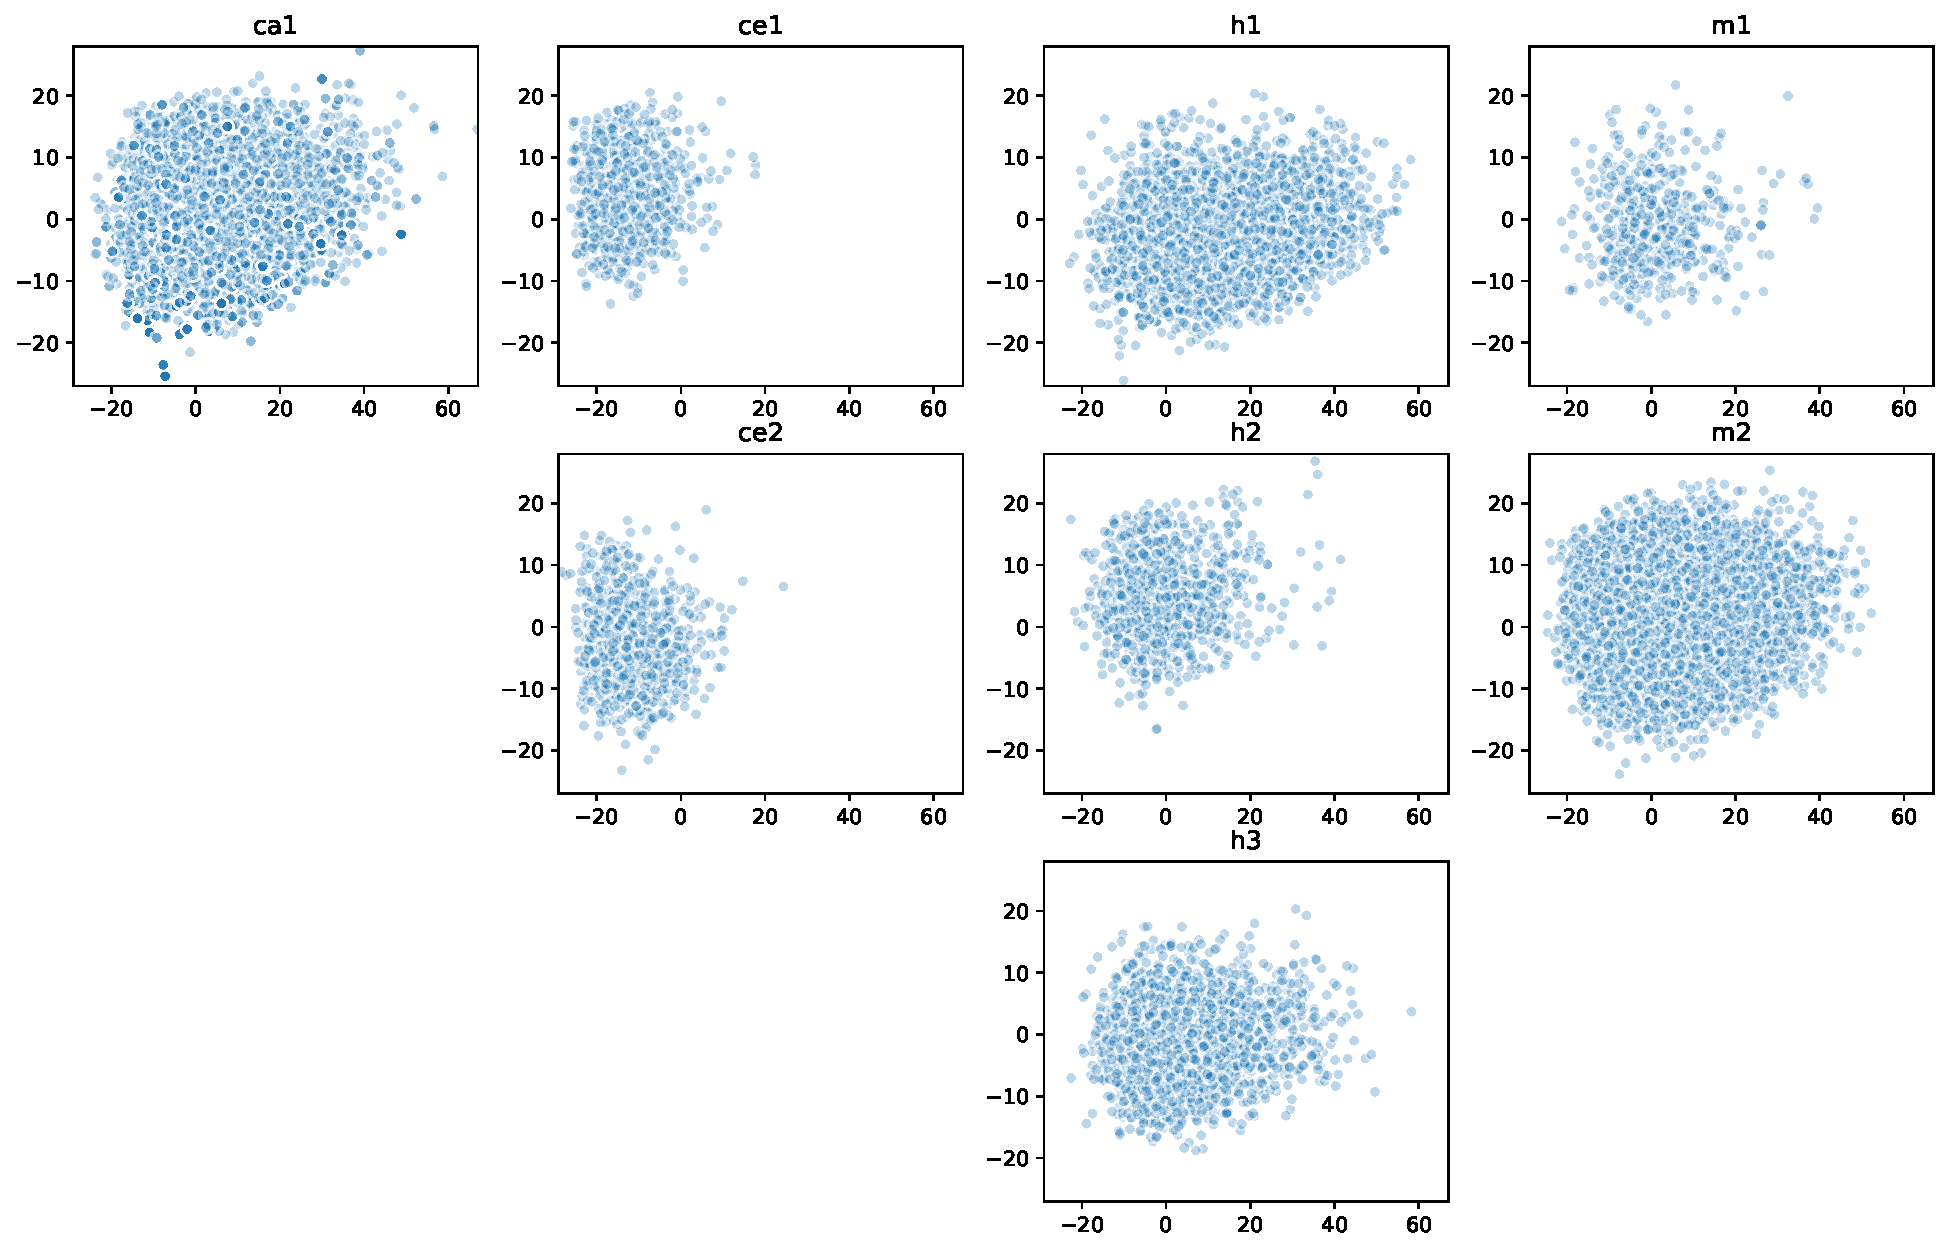
\includegraphics[width = 1\textwidth]{Results/features_pca_with_resample.pdf}
%       \label{fig:feature_pca}
%       \end{figure}

\begin{figure}[h!]
  \caption{\csentence{Datasets presented in 2D.} Each point represents a single interaction after a dimensional reduction of its feature space using PCA. X and Y axes are the first and the second component of the PCA respectively.}
       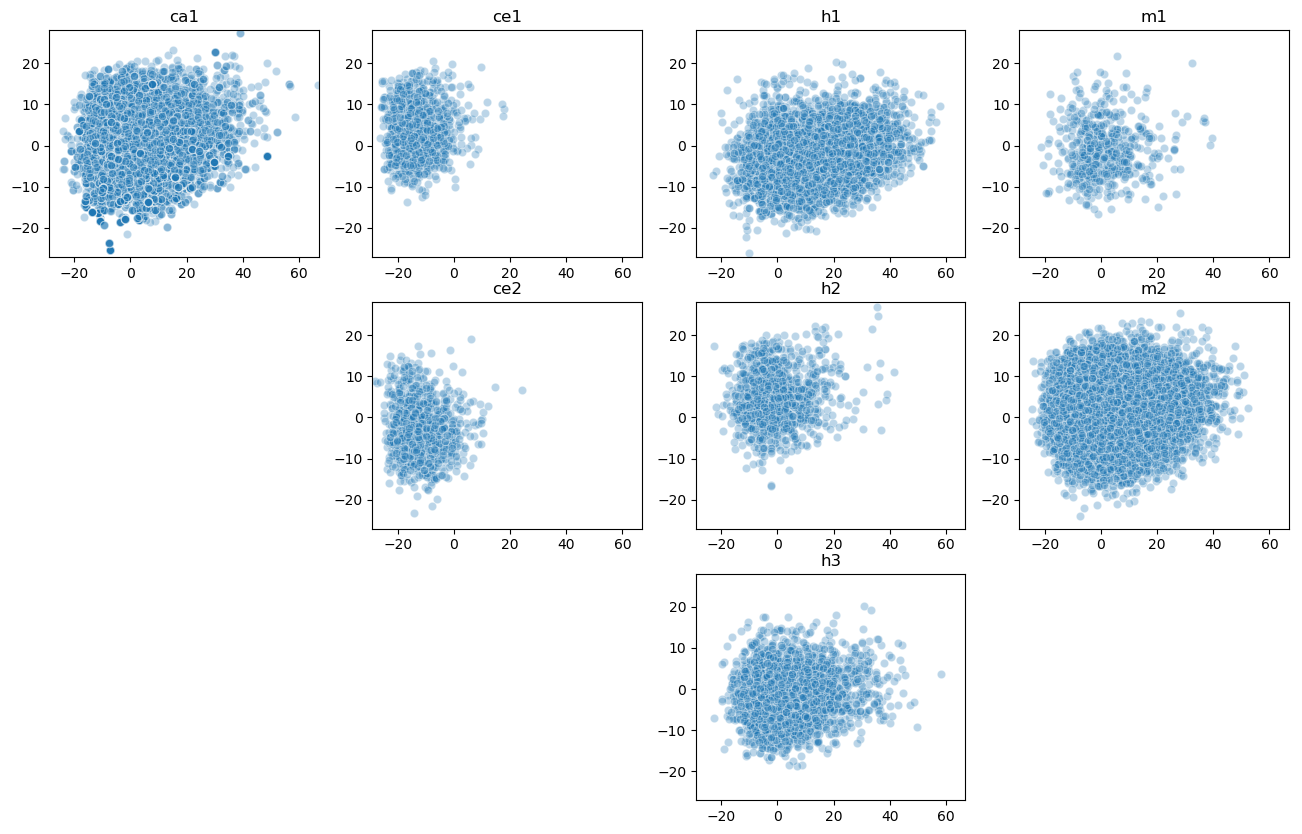
\includegraphics[width = 1\textwidth]{Results/features_pca_with_resample.png}
      \label{fig:feature_pca}
      \end{figure}


\subsection*{Intra-dataset analysis} \label{nameref:indataset}
In this section, we evaluated the performance of machine-learning based binary classifiers to correctly classify positive and negative miRNA-target interactions within the same dataset. 
We first conducted a set of experiments with different types of machine learning classifiers. Then, we performed an in-depth analysis of the best preforming classifier, by measuring different performance metrics and by estimating feature importance.

\subsubsection*{Evaluation of different machine learning methods} \label{sec:evaluation_different_ML}
For each dataset we generated 20 training-testing splits of the data using a stratified random split algorithm. This algorithm ensures that each miRNA appears in the training and the testing sets at the same proportion as in the original dataset.
We then trained 6 widely used classifiers on the 20 training sets of each dataset and measured their performance in the classification of their respective testing sets. We then calculated the average and the standard deviation values of the classification accuracy as shown in Table \ref{tab:self_summary}. Notably, XGBoost classifier achieved the best results across all datasets, with accuracy scores ranging from 0.82 to 0.94, with the following order of performance from low to high: \textit{h1},  \textit{h3},  \textit{m1}, \textit{ce1}, \textit{ce2}, \textit{m2}, \textit{h2}, \textit{ca1}. We did not observe any bias in the ordering of the organisms in the list.   
We compared our results to previous machine learning based approaches that were trained and tested on the human CLASH dataset designated as \textit{h1} in Table \ref{tbl:dataset_description}. The accuracy achieved by our classifiers on this dataset is comparable to the ones reported by previous studies (\nameref{add:figs_tbls}, Table S2). 

\begin{table}[h!]
\caption{Intra-dataset prediction: classification accuracy of different machine learning methods. The cells contain the average and the standard deviation (in brackets) results acquired from 20 models trained and evaluated on different dataset splits.}
\label{tab:self_summary}
\begin{tabular}{|l|l|l|l|l|l|l|}
\hline
Dataset & XGBoost & RF & KNN & SGD & SVM & LR \\ \hline
ca1                               & \begin{tabular}[c]{@{}l@{}}0.937 \\ (0.002)\end{tabular} & \begin{tabular}[c]{@{}l@{}}0.885 \\ (0.004)\end{tabular} & \begin{tabular}[c]{@{}l@{}}0.828 \\ (0.003)\end{tabular} & \begin{tabular}[c]{@{}l@{}}0.797 \\ (0.033)\end{tabular} & \begin{tabular}[c]{@{}l@{}}0.895 \\ (0.003)\end{tabular} & \begin{tabular}[c]{@{}l@{}}0.836 \\ (0.004)\end{tabular} \\ \hline
ce1                               & \begin{tabular}[c]{@{}l@{}}0.889 \\ (0.014)\end{tabular} & \begin{tabular}[c]{@{}l@{}}0.833 \\ (0.019)\end{tabular} & \begin{tabular}[c]{@{}l@{}}0.768 \\ (0.019)\end{tabular} & \begin{tabular}[c]{@{}l@{}}0.798 \\ (0.045)\end{tabular} & \begin{tabular}[c]{@{}l@{}}0.841 \\ (0.015)\end{tabular} & \begin{tabular}[c]{@{}l@{}}0.843 \\ (0.014)\end{tabular} \\ \hline
ce2                               & \begin{tabular}[c]{@{}l@{}}0.891 \\ (0.016)\end{tabular} & \begin{tabular}[c]{@{}l@{}}0.858 \\ (0.018)\end{tabular} & \begin{tabular}[c]{@{}l@{}}0.768 \\ (0.019)\end{tabular} & \begin{tabular}[c]{@{}l@{}}0.819 \\ (0.034)\end{tabular} & \begin{tabular}[c]{@{}l@{}}0.862 \\ (0.012)\end{tabular} & \begin{tabular}[c]{@{}l@{}}0.847 \\ (0.016)\end{tabular} \\ \hline
h1                                & \begin{tabular}[c]{@{}l@{}}0.824 \\ (0.007)\end{tabular} & \begin{tabular}[c]{@{}l@{}}0.769 \\ (0.008)\end{tabular} & \begin{tabular}[c]{@{}l@{}}0.731 \\ (0.007)\end{tabular} & \begin{tabular}[c]{@{}l@{}}0.746 \\ (0.011)\end{tabular} & \begin{tabular}[c]{@{}l@{}}0.795 \\ (0.007)\end{tabular} & \begin{tabular}[c]{@{}l@{}}0.770 \\ (0.007)\end{tabular} \\ \hline
h2                                & \begin{tabular}[c]{@{}l@{}}0.904 \\ (0.007)\end{tabular} & \begin{tabular}[c]{@{}l@{}}0.869 \\ (0.011)\end{tabular} & \begin{tabular}[c]{@{}l@{}}0.857 \\ (0.009)\end{tabular} & \begin{tabular}[c]{@{}l@{}}0.860 \\ (0.03)\end{tabular}  & \begin{tabular}[c]{@{}l@{}}0.879 \\ (0.009)\end{tabular} & \begin{tabular}[c]{@{}l@{}}0.892 \\ (0.009)\end{tabular} \\ \hline
h3                                & \begin{tabular}[c]{@{}l@{}}0.835 \\ (0.007)\end{tabular} & \begin{tabular}[c]{@{}l@{}}0.769 \\ (0.009)\end{tabular} & \begin{tabular}[c]{@{}l@{}}0.744 \\ (0.009)\end{tabular} & \begin{tabular}[c]{@{}l@{}}0.752 \\ (0.034)\end{tabular} & \begin{tabular}[c]{@{}l@{}}0.805 \\ (0.007)\end{tabular} & \begin{tabular}[c]{@{}l@{}}0.795 \\ (0.010)\end{tabular} \\ \hline
m1                                & \begin{tabular}[c]{@{}l@{}}0.847 \\ (0.015)\end{tabular} & \begin{tabular}[c]{@{}l@{}}0.795\\ (0.016)\end{tabular}  & \begin{tabular}[c]{@{}l@{}}0.758 \\ (0.022)\end{tabular} & \begin{tabular}[c]{@{}l@{}}0.760 \\ (0.038)\end{tabular} & \begin{tabular}[c]{@{}l@{}}0.819 \\ (0.019)\end{tabular} & \begin{tabular}[c]{@{}l@{}}0.800 \\ (0.019)\end{tabular} \\ \hline
m2                                & \begin{tabular}[c]{@{}l@{}}0.900 \\ (0.004)\end{tabular} & \begin{tabular}[c]{@{}l@{}}0.826 \\ (0.004)\end{tabular} & \begin{tabular}[c]{@{}l@{}}0.797 \\ (0.004)\end{tabular} & \begin{tabular}[c]{@{}l@{}}0.798 \\ (0.017)\end{tabular} & \begin{tabular}[c]{@{}l@{}}0.873\\ (0.004)\end{tabular}  & \begin{tabular}[c]{@{}l@{}}0.833 \\ (0.004)\end{tabular} \\ \hline
\end{tabular}
\end{table}

% \subsubsection*{In-depth analysis of the xGBoost performance}
% We next sought to perform an in-depth performance analysis of the xGBoost classifier since it achieved the highest accuracy across all datasets (Table \ref{tab:self_summary}). Therefore, we calculated 7 widely used performance metrics including accuracy (ACC), sensitivity (TPR: true positive rate), specificity (TNR: true negative rate), precision (PPV: positive predictive value), negative predictive value (NPV) and the rates of false positives (FPR) and false negatives (FNR) (Table \ref{tab:measurementinfo}). 

\subsubsection*{In-depth analysis of the XGBoost performance}
We next sought to perform an in-depth performance analysis for the XGBoost classifier since it achieved the highest accuracy across all datasets. Therefore, we calculated 8 widely used performance metrics (Table \ref{tab:measurementinfo}). The performance of a good classifier is characterized by high true detection rate (i.e., TPR and TNR close to 1) and low miss-detection rate (i.e., FNR and FPR close to 0). We observed that the TPR and TNR values per dataset are very similar and range in 0.82-0.91 across all datasets. Similarly, the FPR and FNR values are similar per dataset, and range in 0.06-0.19 across all datasets. 

PPV and NPV describe the precision of the classifier: PPV is the proportion of the true positive predictions out of all positive predictions; NPV is the proportion of the true negative predictions from all negative predictions. The values of these measures range from 0 (worst) to 1 (ideal). Our classifiers achieved rates of 0.83-0.95.

Area under the curve (AUC) is a performance measurement for classification problems at different threshold settings. It provides information on the capability of a model to differentiate between classes. AUC values range from 0 to 1, where a model with perfect predictions achieves AUC of 1. Our classifiers achieved AUC score of 0.91-0.98.

Altogether, these metrics indicate that all 8 XGBoost classifiers (corresponding to each dataset) are balanced, accurate and precise. Even though the classifiers for \textit{h1}, \textit{h3} and \textit{m1}, achieved relatively low accuracy performance, they can be still considered as practical for miRNA-target prediction.

\begin{table}[h!]
\caption{XGBoost performance measurements. The cells contain the average and the standard deviation (in brackets) results acquired from 20 models trained and evaluated on different training and testing dataset splits.}
\label{tab:measurementinfo}
  \begin{threeparttable}

\begin{tabular}{|l|l|l|l|l|l|l|l|l|l|}
\hline
Dataset & TPR \tnote{a} & TNR \tnote{b} & PPV \tnote{c} & NPV \tnote{d}
& FPR \tnote{e} & FNR \tnote{f} & ACC \tnote{g} & AUC \tnote{h} \\ \hline
ca1  & \begin{tabular}[c]{@{}l@{}} 0.932 \\ (0.004)\end{tabular} & \begin{tabular}[c]{@{}l@{}} 0.943 \\ (0.004)\end{tabular} & \begin{tabular}[c]{@{}l@{}} 0.943 \\ (0.004)\end{tabular} & \begin{tabular}[c]{@{}l@{}} 0.931 \\ (0.004)\end{tabular} & \begin{tabular}[c]{@{}l@{}} 0.057 \\ (0.004)\end{tabular} & \begin{tabular}[c]{@{}l@{}} 0.068 \\ (0.004)\end{tabular} & \begin{tabular}[c]{@{}l@{}} 0.937 \\ (0.002)\end{tabular} & \begin{tabular}[c]{@{}l@{}} 0.983 \\ (0.001)\end{tabular} \\ \hline
ce1  & \begin{tabular}[c]{@{}l@{}} 0.89 \\ (0.018)\end{tabular}  & \begin{tabular}[c]{@{}l@{}} 0.889 \\ (0.014)\end{tabular} & \begin{tabular}[c]{@{}l@{}} 0.889 \\ (0.015)\end{tabular} & \begin{tabular}[c]{@{}l@{}} 0.89 \\ (0.019)\end{tabular}  & \begin{tabular}[c]{@{}l@{}} 0.111 \\ (0.014)\end{tabular} & \begin{tabular}[c]{@{}l@{}} 0.11 \\ (0.018)\end{tabular}  & \begin{tabular}[c]{@{}l@{}} 0.889 \\ (0.014)\end{tabular} & \begin{tabular}[c]{@{}l@{}} 0.955 \\ (0.009)\end{tabular} \\ \hline
ce2  & \begin{tabular}[c]{@{}l@{}} 0.884 \\ (0.02)\end{tabular}  & \begin{tabular}[c]{@{}l@{}} 0.899 \\ (0.019)\end{tabular} & \begin{tabular}[c]{@{}l@{}} 0.901 \\ (0.02)\end{tabular}  & \begin{tabular}[c]{@{}l@{}} 0.881 \\ (0.023)\end{tabular} & \begin{tabular}[c]{@{}l@{}} 0.101 \\ (0.019)\end{tabular} & \begin{tabular}[c]{@{}l@{}} 0.116 \\ (0.02)\end{tabular}  & \begin{tabular}[c]{@{}l@{}} 0.891 \\ (0.016)\end{tabular} & \begin{tabular}[c]{@{}l@{}} 0.958 \\ (0.012)\end{tabular} \\ \hline
h1   & \begin{tabular}[c]{@{}l@{}} 0.816 \\ (0.008)\end{tabular} & \begin{tabular}[c]{@{}l@{}} 0.833 \\ (0.008)\end{tabular} & \begin{tabular}[c]{@{}l@{}} 0.838 \\ (0.009)\end{tabular} & \begin{tabular}[c]{@{}l@{}} 0.811 \\ (0.01)\end{tabular}  & \begin{tabular}[c]{@{}l@{}} 0.167 \\ (0.008)\end{tabular} & \begin{tabular}[c]{@{}l@{}} 0.184 \\ (0.008)\end{tabular} & \begin{tabular}[c]{@{}l@{}} 0.824 \\ (0.007)\end{tabular} & \begin{tabular}[c]{@{}l@{}} 0.908 \\ (0.006)\end{tabular} \\ \hline
h2   & \begin{tabular}[c]{@{}l@{}} 0.886 \\ (0.012)\end{tabular} & \begin{tabular}[c]{@{}l@{}} 0.924 \\ (0.011)\end{tabular} & \begin{tabular}[c]{@{}l@{}} 0.928 \\ (0.012)\end{tabular} & \begin{tabular}[c]{@{}l@{}} 0.881 \\ (0.014)\end{tabular} & \begin{tabular}[c]{@{}l@{}} 0.076 \\ (0.011)\end{tabular} & \begin{tabular}[c]{@{}l@{}} 0.114 \\ (0.012)\end{tabular} & \begin{tabular}[c]{@{}l@{}} 0.904 \\ (0.007)\end{tabular} & \begin{tabular}[c]{@{}l@{}} 0.972 \\ (0.003)\end{tabular} \\ \hline
h3   & \begin{tabular}[c]{@{}l@{}} 0.823 \\ (0.011)\end{tabular} & \begin{tabular}[c]{@{}l@{}} 0.849 \\ (0.009)\end{tabular} & \begin{tabular}[c]{@{}l@{}} 0.854 \\ (0.011)\end{tabular} & \begin{tabular}[c]{@{}l@{}} 0.816 \\ (0.015)\end{tabular} & \begin{tabular}[c]{@{}l@{}} 0.151 \\ (0.009)\end{tabular} & \begin{tabular}[c]{@{}l@{}} 0.177 \\ (0.011)\end{tabular} & \begin{tabular}[c]{@{}l@{}} 0.835 \\ (0.007)\end{tabular} & \begin{tabular}[c]{@{}l@{}} 0.914 \\ (0.004)\end{tabular} \\ \hline
m1   & \begin{tabular}[c]{@{}l@{}} 0.834 \\ (0.014)\end{tabular} & \begin{tabular}[c]{@{}l@{}} 0.862 \\ (0.024)\end{tabular} & \begin{tabular}[c]{@{}l@{}} 0.866 \\ (0.027)\end{tabular} & \begin{tabular}[c]{@{}l@{}} 0.828 \\ (0.017)\end{tabular} & \begin{tabular}[c]{@{}l@{}} 0.138 \\ (0.024)\end{tabular} & \begin{tabular}[c]{@{}l@{}} 0.165 \\ (0.014)\end{tabular} & \begin{tabular}[c]{@{}l@{}} 0.847 \\ (0.015)\end{tabular} & \begin{tabular}[c]{@{}l@{}} 0.914 \\ (0.007)\end{tabular} \\ \hline
m2   & \begin{tabular}[c]{@{}l@{}} 0.891 \\ (0.003)\end{tabular} & \begin{tabular}[c]{@{}l@{}} 0.909 \\ (0.005)\end{tabular} & \begin{tabular}[c]{@{}l@{}} 0.911 \\ (0.006)\end{tabular} & \begin{tabular}[c]{@{}l@{}} 0.888 \\ (0.003)\end{tabular} & \begin{tabular}[c]{@{}l@{}} 0.091 \\ (0.005)\end{tabular} & \begin{tabular}[c]{@{}l@{}} 0.109 \\ (0.003)\end{tabular} & \begin{tabular}[c]{@{}l@{}} 0.9 \\ (0.004)\end{tabular}  & \begin{tabular}[c]{@{}l@{}} 0.963 \\ (0.002)\end{tabular} \\ \hline
\end{tabular}
\begin{tablenotes}\footnotesize
\item[a] True Positive Rate (Sensitivity)
\item[b] True Negative Rate (Specificity)
\item[c] Positive Predictive Value (Precision)
\item[d] Negative predictive Value
\item[e] False Positive Rate (Fall out)
\item[f] False Negative Rate
\item[g] Overall accuracy
\item[h] Area Under the Receiver Operating Characteristic Curve
\end{tablenotes}
  \end{threeparttable}
\end{table}

%   # Sensitivity, hit rate, recall, or true positive rate
%     "TPR" : TP / (TP + FN),
%     # Specificity or true negative rate
%     "TNR" : TN / (TN + FP),
%     # Precision or positive predictive value
%     "PPV" : TP / (TP + FP),
%     # Negative predictive value
%     "NPV" : TN / (TN + FN),
%     # Fall out or false positive rate
%     "FPR" : FP / (FP + TN),
%     # False negative rate
%     "FNR" : FN / (TP + FN),
%     # False discovery rate
%     "FDR" : FP / (TP + FP),
%     # Overall accuracy
%     "ACC" : (TP + TN) / (TP + FP + FN + TN),


\subsubsection*{Random split control}
In the above analysis, the splitting of the dataset into the training and testing sets was done in a way that preserves the miRNA distribution in both sets (stratified split). To assess how this type of split affects the classifier performance, we repeated the analysis with the XGBoost classifier, but this time used a random split strategy (control split) to generate the training and the testing sets. Our results showed that there is almost no difference between the results achieved with the stratified and the control split methods. The accuracy results for the control splits are found in \nameref{add:figs_tbls}, Table S3.

\subsubsection*{Top important features of each dataset}
We used 490 features in order to describe the interactions. We next sought to identify the top important features of each dataset, their relative scores, and the degree of overlap of the top features between different datasets. XGBoost classifier reports a list of five feature importance metrics: weight, gain, cover, total gain and total cover. We extracted the 5 metrics for all 20 train-test splits of each dataset and calculated their mean and standard deviation (\nameref{add:feature importance}, Table S7).
For further analysis, we chose the gain metric, which reflects for each feature its contribution to the model. For each dataset, we sorted in descending order, the average features' gain score over all 20 runs, and plotted the curves of all the datasets together.
Figure \ref{fig:feature_importance}a reveals that the gain score is decaying very fast. The 6 top features are significantly stronger relative to the rest (Figure \ref{fig:feature_importance}b). We thus extracted the top 6 features from each dataset, along with their normalized gain score (see methods), into a unified list. The unified list consisted of a total of 16 features (out of the maximum length of 48), indicating that there are many shared features among the datasets. Table \ref{tab:feature_importance} shows the features ordered by their mean gain across all datasets.
Notably, features related to the seed region (marked as bold in the table), comprise half of the features in the table. This finding emphasizes the role of the seed region in the formation of miRNA-mRNA interactions.

\begin{table}[h!]
\caption{Feature importance. The table shows 16 features, which represent the union of the top 6 features of each dataset, along with their gain values which were computed by XGBoost. The values were normalized to the range of (0, 100). The features are ordered by their mean gain across all datasets. For the un-normalized version of the table, see \nameref{add:figs_tbls}, Table S5.}
\label{tab:feature_importance}
\begin{tabular}{|l|l|l|l|l|l|l|l|l|l|}
\hline
\textbf{Feature/Dataset}                          & \textbf{ca1} & \textbf{ce1} & \textbf{ce2} & \textbf{h1} & \textbf{h2} & \textbf{h3} & \textbf{m1} & \textbf{m2} & \textbf{mean} \\ \hline
\textbf{miRNAPairingCount\_Seed\_GU}              & 100          & 87           & 95           & 29          & 40          & 100         & 28          & 100         & 72            \\ \hline
\textbf{miRNAMatchPosition\_1}                    & 63           & 79           & 34           & 70          & 25          & 30          & 27          & 85          & 52            \\ \hline
miRNAPairingCount\_Total\_GU                      & 42           & 71           & 32           & 100         & 19          & 53          & 35          & 28          & 48            \\ \hline
MRNA\_Target\_G\_comp                             & 12           & 74           & 12           & 12          & 36          & 33          & 100         & 37          & 39            \\ \hline
Energy\_MEF\_Duplex                               & 13           & 45           & 11           & 10          & 100         & 19          & 35          & 52          & 36            \\ \hline
\textbf{Seed\_match\_compact\_interactions\_2\_7} & 42           & 33           & 100          & 12          & 18          & 36          & 13          & 18          & 34            \\ \hline
MRNA\_Target\_GG\_comp                            & 30           & 21           & 10           & 12          & 7           & 30          & 79          & 26          & 27            \\ \hline
\textbf{miRNAMatchPosition\_4}                    & 8            & 100          & 21           & 10          & 11          & 16          & 2           & 12          & 22            \\ \hline
miRNAPairingCount\_X3p\_bulge\_nt                 & 3            & 60           & 6            & 25          & 32          & 9           & 9           & 8           & 19            \\ \hline
\textbf{miRNAMatchPosition\_2}                    & 8            & 42           & 37           & 7           & 11          & 13          & 15          & 6           & 17            \\ \hline
\textbf{miRNAMatchPosition\_5}                    & 12           & 27           & 14           & 14          & 6           & 15          & 29          & 12          & 16            \\ \hline
\textbf{miRNAPairingCount\_Seed\_GC}              & 7            & 22           & 24           & 18          & 12          & 13          & 11          & 12          & 15            \\ \hline
miRNAPairingCount\_X3p\_GC                        & 4            & 27           & 11           & 10          & 27          & 8           & 6           & 5           & 12            \\ \hline
Acc\_P21\_10th                                    & 9            & 19           & 7            & 6           & 25          & 7           & 12          & 7           & 11            \\ \hline
Energy\_MEF\_local\_target\_normalized            & 8            & 11           & 6            & 7           & 8           & 11          & 36          & 6           & 11            \\ \hline
\textbf{Seed\_match\_compact\_mismatch\_inner}    & 4            & 3            & 15           & 19          & 0           & 13          & 2           & 9           & 8             \\ \hline
\end{tabular}
\end{table}


\begin{figure}[h!]
    \centering
    \subfloat[Full view of datasets' feature importance]{{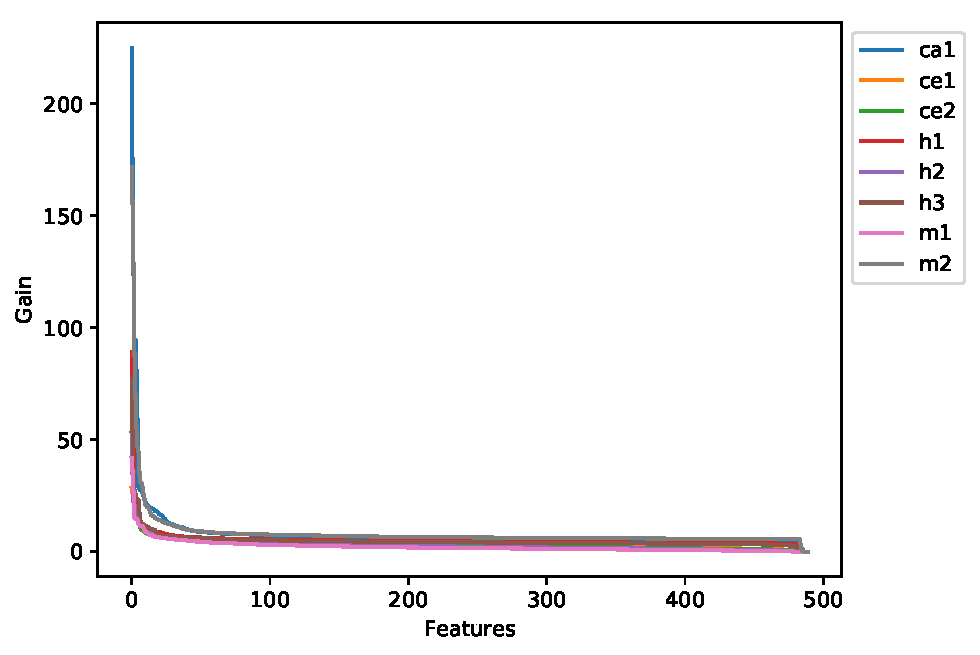
\includegraphics[width=5cm]{Results/feature_importance_full.pdf} }}%
    \qquad
    \subfloat[View of the top 20 features score]{{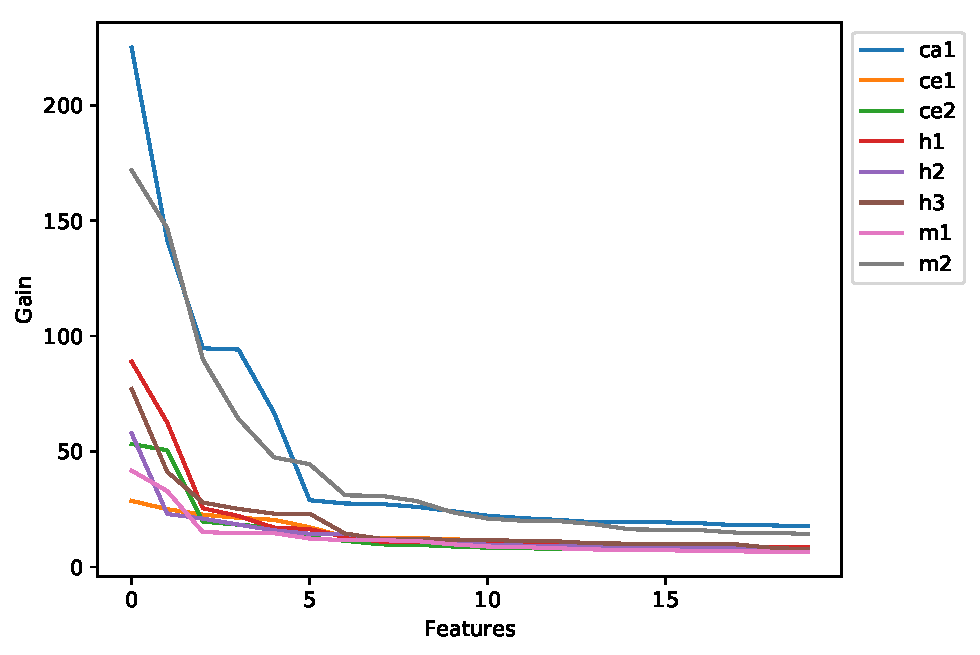
\includegraphics[width=5cm]{Results/feature_importance_zoom.pdf} }}%
    \caption{\csentence{Datasets' feature importance plot}. The figures show the features' gain score. The features are sorted in descending order from the top feature (highest gain) to lowest. Figure (a) shows a full view of the gain plot, and emphasizes the gain decay.  Figure (b) is a zoomed view, focusing on the top 20 features.}%
    \label{fig:feature_importance}%
\end{figure}

\subsection*{Cross-dataset analysis}
In the previous section, we trained, optimized and evaluated the performance of a dedicated classifier for each dataset. In this section, our goal is to examine the relationships between datasets. Thus, we first use a statistical measure to calculate the distance between the datasets. Second, we evaluate the performance of each classifier to properly classify interactions in the other datasets.

\subsubsection*{Kullback–Leibler divergence}
We hypothesized that pair of datasets, with similar characteristics, might achieve better results in classifying the interactions of each other. We thus looked for a measure to assess the level of similarity of a pair of datasets, that will take into account the directionality of the classification task: classifier is trained on one dataset (source) and is applied to classify a second dataset (target).
We chose the asymmetric measure Kullback–Leibler (KL) divergence which measures how the target's probability distribution is different from the probability distribution of the source. KL divergence has its origins in information theory. The primary purpose of the theory of information is to quantify the amount of information in the data. KL divergence measures the information loss when approximating the target distribution by the source distribution. We used KL divergence to measure the pairwise information loss between every two datasets based on their miRNA seed family distribution.

Figure \ref{fig:divergence} shows the divergence between all dataset pairs. The divergence of a dataset with itself is zero, and the divergences between datasets within the same organisms are usually lower than the divergences between different organisms. Notably, the divergence between \textit{C.elegans} datasets, both as targets and as sources, and the other datasets is significantly higher than the divergence between other pairs. The asymmetry of this measure can be observed for example for the pair \textit{(h1,h3)}, for which KL(h1,h3)=1.6 and the KL(h3,h1)=2.1. Intuitively, this means that by provided the seed distribution of dataset \textit{h1}, the information obtained by observing dataset \textit{h3} is smaller than the information received by switching the pair.

\begin{figure}[h!]
  \caption{\csentence{Kullback–Leibler divergence.} Each cell represents the divergence between the source and the target datasets, based on their miRNA seed family distributions. The black frames surround the results of dataset pairs originating from the same organism.}
      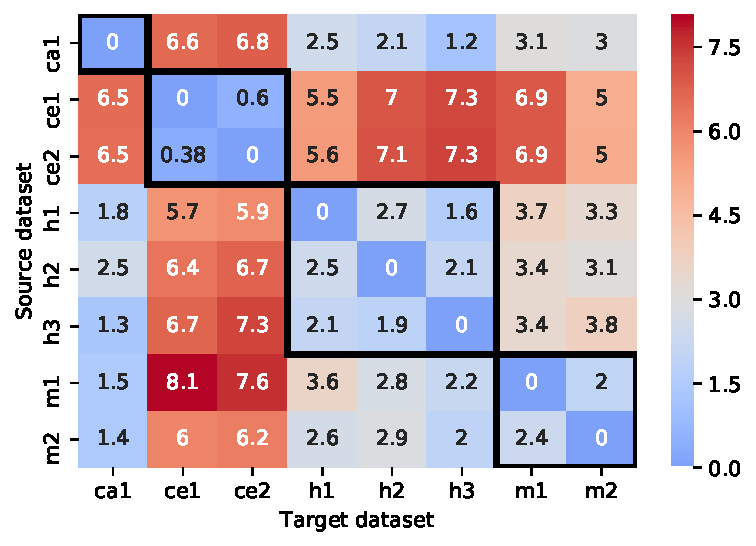
\includegraphics[width = 1\textwidth]{Results/divergence.pdf}
      \label{fig:divergence}
      \end{figure}


\subsubsection*{Classification performance between datasets}
We evaluated the performance of cross dataset miRNA-target predictions, i.e., the performance of a classifier when applied on interactions from datasets different from the the one it was trained on.
We examined all possible 56 combinations, considering each dataset both as a training and as a testing set. 
For each dataset, we loaded the 20 XGBoost classifiers that we trained in section \nameref{nameref:indataset} and used them to classify the rest 7 datasets. Figure \ref{fig:crossdataset} shows the average accuracy over the 20 tests. 

Inspection of the results reveals that there is a variability in the classification performance among the pairs (not including the diagonal), ranging from random, slightly above 0.5, to 0.91. The accuracy matrix is not symmetric, i.e., a pair where a dataset \textit{i} serves as training set and dataset \textit{j} serves as testing set, achieves a different performance than a swapped pair. Pairs of datasets originating from the same organism (surrounded by black boxes in Figure \ref{fig:crossdataset}), generally achieved high accuracy. Intriguingly, the human pairs \textit{(h2,h1)}, \textit{(h2,h3), \textit{(h3,h1)}} achieved a relatively low accuracy score. The low performance of these pairs could be potentially explained by the differences in datasets' size and diversity. In particular, the dataset \textit{h2} is smaller and less diverse then the datasets \textit{h1,h3} (Figure \ref{fig:feature_pca}), and thus a model that uses it as training set achieves lower performance. In most of the cases, the KL divergence results coincide with the accuracy results. For example, for the pair \textit{(h1,h3)}, the KL(h1,h3)=1.6$<$KL(h3,h1)=2.1 and ACC(h1,h3)=0.79$>$ACC(h3,h1)=0.69 demonstrate that dataset \textit{h1} better represents dataset \textit{h3} and as such achieved better accuracy results than vice versa. Interestingly, the KL(h1,h2)=2.5$\approx$KL(h2,h1)=2.7 however ACC(h1,h2)=0.86 while ACC(h2,h1)=0.58. This indicates that there are more factors that affect the ability to predict, such as the dataset's size and  the pattern of interaction appear in the dataset.

Pairs of datasets originating from different organisms, and include \textit{C.elegans} as either a training or a testing set achieved poor performance, ranging from 0.56 to 0.78. The divergence values of these pairs are 2x-4x bigger (ranges from 5 to 8) than the values of other pairs, indicating that seed distributions of other organisms poorly represent the \textit{C.elegans} datasets and vice versa. Other pairs of two organisms achieve much higher accuracy, reaching up to a 0.91. Lowest accuracy in these mixed pairs was observed for pairs that contained \textit{h1} as a testing set. Notably, this dataset was used by previous methods (\nameref{add:figs_tbls}, Table S1) for training/testing purposes only, and has never been evaluated as independent testing set.     

% To summarize, the \textit{C.elegans} datasets achieve good performance inside their own group and a bad performance with datasets from other organisms. Datasets from human, mouse and cattle the rest  On the other hand, most of the accuracy results between the rest organisms are above 80\%, which is similar to the accuracy performance of target-prediction algorithms from human to human. 

Additional  factors that influence the accuracy will be further discussed in the discussion section.


\begin{figure}[h!]
  \caption{\csentence{Cross dataset accuracy results}. Cell (i,j) represents the accuracy result of a classifier that was trained on dataset \textit{i} and tested on dataset \textit{j}. Each cell shows the average accuracy over the 20 trained classifiers generated for each dataset in section \nameref{sec:evaluation_different_ML}. The black frames surround the results of dataset pairs originating from the same organism. The accuracy result for predicting the dataset itself, was taken from section \nameref{nameref:indataset}. }
      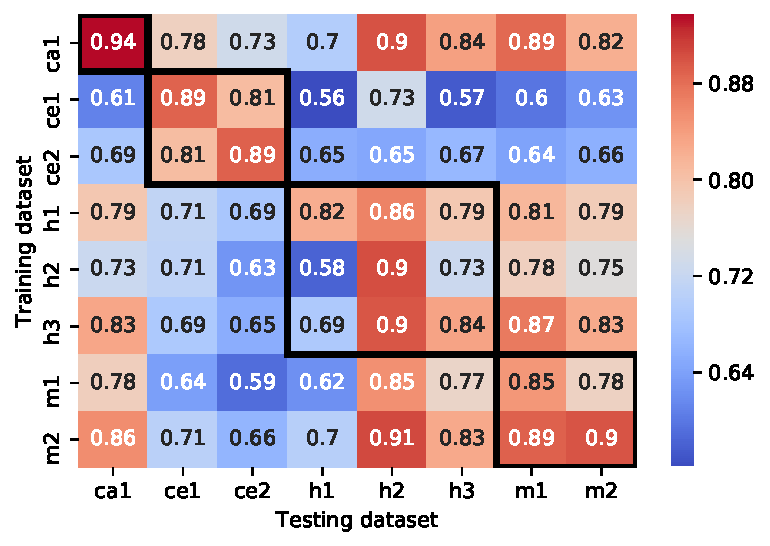
\includegraphics[width = 1\textwidth]{Results/diff_summary.pdf}
    \label{fig:crossdataset}
      \end{figure}

%%%%%%%%%%%%%%%%%%%%%%%%%%%%%%%%%%%%%%%%%%%%%%%%%%%%%%%%%%%%%%%%%%%%%%%%%%%%%%%%%
%%%%%%%%% Discussion %%%%%%%%%%%%%%%%%%%%%%%%%%%%%%%%%%%%%%
%%%%%%%%%%%%%%%%%%%%%%%%%%%%%%%%%%%%%%%%%%%%%%%%%%%%%%%%%%%%%%%%%%%%%%%%%%%%%%%%%
\clearpage
\section*{Discussion}
Identifying miRNA target sites on mRNAs is a fundamental step in understanding miRNA function. A notable progress in this task has been achieved due to novel experimental protocols, availability of high-throughput unambiguous miRNA-target datasets and adoption of advance machine learning methods in target prediction models. Several studies applied classic machine learning \cite{lu2016learning, ding2016tarpmir, wang2016improving, liu2019prediction} and deep learning \cite{wen2018deepmirtar, paker2019mirlstm, pla2018miraw} methods on some of these datasets advancing the field towards more accurate prediction. Our goal in this study was to assess the transferability of miRNA-target rules between organisms. Furthermore, we sought to understand how different characteristics of the training and the testing sets affect the performance of miRNA-target prediction models. To this end we performed a comparative analysis of available miRNA-target chimeric datasets, and applied machine learning approaches to address these goals.

\subsection*{Available data}
The availability of large and high-quality data is crucial for a machine learning based research. In the field of experimental miRNA-target identification, several approaches to generate high-throughput datasets are available. Most common approach is based on measuring mRNA expression changes in miRNA overexpression experiments in cell culture, however it has several major problems \cite{li2019current, martinez2013microrna}. First, such data may contain indirect signals of regulation. Second, for direct regulation, the exact binding sites are unknown and have to be predicted within the whole 3'UTR or even the whole mRNA sequence. Furthermore, such experimental settings may represent a non-physiological context for miRNA activity and may not accurately reflect endogenous targeting rules. Finally, it may miss signals of translation efficiency inhibitions that is not reflected in changes of mRNA levels \cite{fabian2010regulation}.

Recently developed methods for Argonaute protein cross-linking and immunoprecipitation (AGO-CLIP) enable experimental identification of thousands of transcriptome wide precise miRNA binding sites \cite{chi2009argonaute, hafner2010transcriptome,zisoulis2010comprehensive}. However, these methods do not provide the identity of the miRNA that is bound to each binding site. Computational algorithms usually resolve these uncertainties by identifying which highly expressed miRNAs are associated with individual AGO-CLIP peaks \cite{majoros2013microrna, reczko2012functional, liu2013clip, khorshid2013biophysical}.

In more advanced methods, e.g., CLASH \cite{helwak2013mapping}, crosslinking and immunoprecipitation are followed by an RNA ligation step, leading to unambiguous determination of chimeric miRNA-target site pairs. These chimeric datasets contain many non-canonical interactions that enrich the repertoire of miRNA-target interactions. However, the main limitation of these methods is the low yield of chimeric reads that are being recovered (around $\sim 2$\%), suggesting that a large number of miRNA-mRNA interactions remains uncaptured. \\

In our analysis we chose to focus on chimeric miRNA-target datasets, as these provide direct evidence for miRNA and specific target site interactions. We utilized eight available chimeric datasets from four organisms. The available datasets were originated from variety of tissues or developmental stages, and were generated by different experimental protocols, including AGO-CLIP with endogenous ligation. During the collection of the datasets, we encountered different data formats. Thus, we developed a processing pipeline which transforms them to the same format. This pipeline is a powerful infrastructure which will enable us, with a relatively low effort, to add more data sources to the analysis in the future, when these become available. 
Our processing pipeline produced final datasets with variable sizes: four small datasets, two large datasets and two massive datasets. Of note, all the presented analyses were performed on the final dataset sizes, except for the PCA analysis in which we used an oversampling method to adjust the sizes.

\subsection*{Thorough analysis of the datasets}
We conducted statistical analyses and visualized datasets from various perspectives, treating each dataset on its own as well as in a comparative manner. 
Our analysis of frequencies of miRNA sequences revealed that there are differences in miRNA sequence distributions among datasets, even if they originated from the same organism. In addition, each dataset is dominated by a small set of miRNA sequences (30-50\% of most frequent miRNAs comprise 90\% of the interactions). These distributions mirror the distributions inside the cells, as it was reported that miRNA frequency in miRNA-target chimeras is correlated with total miRNA abundance \cite{darnell_moore2015mirna}.

We continued by categorizing the interactions based on their seed type (canonical and non-canonical) and base-pairing density. Perfect seed complementary (referred as canonical seeds) between target sites and miRNA seed sequences (nts 2-7 or 2-8), has long been recognized as a critical dominant feature for miRNA targeting \cite{bartel2009micrornas, lewis2005conserved}. Nevertheless, in recent years we witnessed several examples of functional miRNA-target interactions that occur without perfect seed pairing, featuring GU pairs, mismatches and bulges in the seed region (referred as non-canonical seeds). Examples include the well-established let-7 targeting of lin-41 in \textit{C.elegans} \cite{slack2000lin, vella2004c}, with one site containing one-nucleotide bulge in the target, and the other site containing a GU pair. Moreover, non-canonical miRNA-target sites called “nucleation bulges”, where the target sites matched to the seed (positions 2-7) contained a bulged-out G nucleotide corresponding to position between 5 and 6 of the miRNA, were identified for miR-124 when analyzing AGO HITS-CLIP data from mouse brain \cite{chi2012alternative}. However, the functionality of non-canonical sites is still a matter of debate, since a recent analysis of non-canonical target sites revealed that even though these sites are bound by the miRNA complex, they do not appear to be broadly functional \cite{agarwal2015predicting}. 

We showed that majority of the interactions in most datasets are non-canonical (48-70\%). Furthermore, in both canonical and non-canonical groups, a large fraction of interactions is characterized by medium and high density of base-pairing (11-16 and more than 16 base-pairs, respectively), predicting the existence of additional pairing beyond the seed region. These auxiliary non-seed interactions were suggested to compensate and stabilize imperfect seed matches \cite{brennecke2005principles, grimson2007microrna}. Moreover, non-seed interactions, were also shown to contribute to target specificity among miRNA seed family members (same seed, divergent non-seed sequence), both in the case of canonical and non-canonical seeds \cite{broughton2016pairing, darnell_moore2015mirna}.\\

To be able to visualize the datasets by their features, we transformed the datasets into 2 dimensions using PCA. Visualization of the transformed data highlighted datasets with lower spread. In particular, \textit{C.elegans} datasets are exceptional relative to rest of the organisms, showing concentration in a narrower area. In addition, the datasets \textit{m1} and \textit{h2}, that represent endogenously ligated chimeras from a mixture of AGO-CLIP experiments, are relatively smaller in size compared to other datasets from the same organism and have lower spread. The exception of these two datasets may explain the lower accuracy results obtained in cross-datasets experiments  when we used them as training sets.
% Isana's comment: Logically, it should not affect the results when they are used as testing set, right? I checked the results, when looking just inside human - it is bad only when used as training, and pretty good when a testing. As for mouse m1->m2 is much lower than m2->m1 -- so we can omit the "testing" in the sentence.

\subsection*{Features and their significance}
Recent studies, especially those that are based on deep learning (e.g., \cite{wen2018deepmirtar}), suggested classifiers that were trained on a large number of features, including high-level and low-level expert-designed and raw-data-level features. Raw-data-level features encode the sequence of the miRNA and the target site. In our study, we used 490 various features to describe the interactions, enabling the model to identify and learn different interaction patterns. 

However, we did not include the previously suggested raw-data-level features, in order to avoid potential information-leakage from the training set to the testing set. First, we saw that the seed families are not uniformly distributed. Second, in our study, the negative sequences are synthetically generated such that there is no match in the seed region to any known miRNA. Thus, including these features could lead the machine learning model to learn to distinguish between real and mock miRNA seeds.  Moreover, in such case, the model may be over-fitted and fail to generalize the rules of interactions. Indeed, and perhaps not surprisingly, we have achieved higher classification performance when we included the raw-data-level features in our models (\nameref{add:figs_tbls}, Table S4). The authors of another study \cite{pla2018miraw}, that did use raw sequence features, addressed this issue by generating a negative dataset based on experimentally verified data instead of mock miRNAs. A comparison between different methods for the generation of negative datasets is an interesting direction for future research. In particular, the evaluation of how the combination of these methods and different feature sets affects the performance of miRNA-target prediction classifiers would help to generate standard approaches for future studies.

% Previous works represent the interactions within the seed site as nominal categorical data. As such, there is no concept of ordering amongst the values represent by these features. Therefore, we designed 13 features to represent the interactions and the relationships between them (e.g., the pair 6mer1GU4$\leftrightarrow$6mer1GU5 is closer than the pair 6mer1GU4$\leftrightarrow$6mer1GU6). Indeed, some of the these new feature ranked high in the feature importance analysis.

The feature importance analysis revealed that there is a small group of features which are significantly dominant. Even though the analysis identified the features for each dataset independently, we showed that there is a significant overlap between the groups, and the unified group contains only 16 features. Importantly, half of these features are seed-related, reiterating the significance of this region in miRNA-target interactions \cite{agarwal2015predicting}.

Some of the datasets are relatively small, with low ratio of interactions to features. For \textit{ce1, ce2, h2} the ratio is $\sim$4, and for \textit{m1} it is $\sim$2. Low ratio can produce models with high bias and high variance. In general, reduction in the number of features, when possible, was shown to be a successful practice. In this work, some of the features are highly correlated, thus can be combined. There are a number of methods for feature selection and dimensionality reduction that may be evaluated in the future. As a preview, we used a basic method of feature selection, based on the XGBoost feature importance data. We used 16 features taken from table \ref{tab:feature_importance} and repeated the analysis (\nameref{add:figs_tbls}, Table S6, Figure S2). The results were similar to the results obtained when all features were included, indicating that a future research that will evaluate different dimensionality reduction methods should be considered to optimize the classification models. 

\subsection*{Intra-dataset analysis}
\subsubsection*{Training and testing split} 
The splitting procedure of the data into training and testing sets has a crucial role in the evaluation of machine learning models. In the miRNA-target prediction task, there is no pre-defined split to training and testing sets as is usually common in other fields, for example, in computer vision (e.g., MNIST \cite{mnist10027939599}). Therefore, we used three strategies to reduce the effect of the split on our results: (1) using stratified training-testing split which ensures the same distribution of miRNA sequences in both training and testing sets; (2) generating control sets by pure-random split algorithm and (3) generating for the above split approaches several training and testing sets using different random states and reporting the mean and the standard deviation values of the results. Indeed, we got similar results with both splitting methods and very low standard deviation values, reassuring that the split strategies did not bias our results.

\subsubsection*{Using tree-based classifier} 
For our thorough analysis, we used XGboost \cite{xgboost}, which is one of the leading gradient boosting tree-based tools for classification \cite{nielsen2016tree}. Differently from deep-learning, XGboost is less computationally expensive and usually does not require a GPU for training, and it can work both with small and large datasets. Additionally, XGboost provides the ability to evaluate and explain the classification rules and rank the features by their importance. 
We showed that XGboost achieved the best performance over the statistical machine learning algorithms (e.g., SVM and LR) for all datasets. Furthermore, it achieved comparable results with respect to deep learning algorithms that were previously applied on the human dataset \textit{h1} \cite{wen2018deepmirtar, lee2016deeptarget}.

\subsection*{Cross-dataset analysis}
Most of the previous works trained and tested their predictive models based on a single chimeric miRNA-target dataset (usually \textit{h1}), sometimes complemented by additional experimental data from databases (e.g., \cite{xiao2009mirecords,chou2016mirtarbase}) or AGO-CLIP data \cite{ding2016tarpmir,wen2018deepmirtar,paker2019mirlstm, lu2016learning, pla2018miraw}. Then these models were evaluated on portions taken out from the training set and in some cases on a few independent datasets from the same or other organisms  (\nameref{add:figs_tbls}, Figure S1). 
The contribution of our work is in providing for the first-time a thorough analysis of all available miRNA-target chimeric datasets, outlining their similarities and dissimilarities. Additionally, we explored the ability to learn classification rules from one dataset and apply them on another dataset, considering all possible combinations of dataset pairs.

The accuracy results of cross-dataset classification ranged between 0.56 to 0.94. To be able to explain these results we examined several factors. First, we estimated the evolutionary distance for every pair of organisms (i.e., the time since the organisms diverged from their common ancestor (Table \ref{tab:evolutiontime})). Among our organisms, the mouse and the human are the closet organisms, then cattle is equally and relatively close to them, while \textit{C.elegans} is the most distant from all. Indeed, we got highest accuracy results when we trained-tested datasets of the same organism, and the lowest accuracy results when trained-tested combinations of \textit{C.elegans} datasets with those from other organisms.

Second, we measured the Kullback–Leibler (KL) divergence for every pair of datasets based on their miRNA seed family distribution. Interestingly, and maybe not surprisingly, the KL divergence results coincide with the evolutionary distance of the organisms, where \textit{C.elegans} datasets exhibit the highest distance from the datasets of other organisms. The divergence within the same organism is, on average, lower than the divergence between different organisms. This divergence is probably associated with the differences in miRNA distributions among different cell types or developmental stages from which the datasets were generated (Table \ref{tbl:dataset_description}). The high correlation that we observe between KL-divergence and the classification performance, reiterates the significance of the seed region in miRNA-target interactions.

Third, we examined the ratio of dominant miRNAs in the dataset. Previous analysis of chimeric datasets showed that individual miRNAs exhibit enrichment for specific classes of base-pairing patterns \cite{helwak2013mapping, broughton2016pairing}, suggesting that they may follow different targeting rules. Thus, high ratio of dominant miRNAs in the dataset, may lead the machine learning model to focus on learning their rules. The cross-dataset results reflected the ability of the model to generalize these rules into universal interaction rules. Additional factors, such as the training dataset size, the experimental protocol and the diversity of the interactions (reflected by the covered area in the PCA plots) could also contribute to the observed results. \\


\begin{table}[h!]
\caption{Estimated divergence time {[}MYA{]} between organisms in our study. Each cell represents the time since the pair of organisms from the corresponding row and column diverged from their common ancestor (source: \cite{kumar2017timetree}).}
\label{tab:evolutiontime}
\begin{tabular}{|l|l|l|l|}
\hline
%              & Mus & Bos taurus & Caenorhabditis elegans \\ \hline
% Homo sapiens & 90  & 96         & 797                    \\ \hline
% Mus          &     & 96         & 797                    \\ \hline
% Bos taurus   &     &            & 797                    \\ \hline
             & Mouse & Cattle & C.elegans \\ \hline
Human & 90  & 96         & 797                    \\ \hline
Mouse          &     & 96         & 797                    \\ \hline
Cattle   &     &            & 797                    \\ \hline
\end{tabular}
\end{table}

\subsection*{Conclusions and future perspectives}
The accuracy results we have got in our cross-datasets experiments are very high, as long as the organisms are within a certain evolutionary distance. These results suggest that target prediction models could be applied also to organisms where experimental training data is limited or unavailable, as long as they are close enough to the organism that is used for training.
As more datasets become available, they could be processed with our pipeline and incorporated into the cross-dataset analysis. Expansion of such analysis on more datasets in the future may also provide insights about the evolution of miRNA-targeting, and identification of general, as well as, organism-specific features. Another interesting research direction will be to combine the information from several datasets in an iterative manner and examine the prediction accuracy in close and more distant organism.

%%%%%%%%%%%%%%%%%%%%%%%%%%%%%%%%%%%%%%%%%%%%%%%%%%%
%%%%%%%%%%%%%%%%%%%%%%%%%%%%%%%%%%%%%%%%%%%%%%%%%%%
% Materials and methods
%%%%%%%%%%%%%%%%%%%%%%%%%%%%%%%%%%%%%%%%%%%%%%%%%%%
%%%%%%%%%%%%%%%%%%%%%%%%%%%%%%%%%%%%%%%%%%%%%%%%%%%

\clearpage
\section*{Materials and methods}
\subsection*{Software packages and tools}
Code developed under this research was implemented as a Python package running on a Linux platform. It uses bioinformatics, data analysis and machine learning packages. The bioinformatics packages are ViennaRNA Package \cite{lorenz2011viennarna}, Biopython (v1.72) \cite{cock2009biopython} and NCBI Blast \cite{altschul1990basic_blast}. The data packages are pandas (v0.23.4) \cite{mckinney2010data_pandas} and numpy (v1.15.4) \cite{oliphant2006guide_numpy}. The machine learning packages are scikit-learn (v0.20.1) \cite{pedregosa2011scikit} and XGBoost (v0.81) \cite{xgboost}.

\subsection*{Data processing}
We acquired eight high-throughput chimeric miRNA-target  datasets from four different organisms: human, mouse, cattle and worm (Table \ref{tbl:dataset_description}). The datasets' files were downloaded from the journals' websites \cite{scheel2017global, grosswendt2014unambiguous, broughton2016pairing, helwak2013mapping, darnell_moore2015mirna}. In addition, we downloaded miRNA sequences from miRBase (releases 17-22) \cite{kozomara2013mirbase} and 3'UTR sequences from Ensembl Biomart database \cite{smedley2015biomart}. Genomic sequences for \textit{C.elegans} were downloaded from wormBase \cite{lee2017wormbase}, and for human and mouse from UCSC Genome Browser \cite{karolchik2004ucsc}.
The datasets were provided in different formats, containing different levels of information about the interactions. Therefore, we developed a processing pipeline to transform the datasets into a standard format, and to include the following fields: metadata (interaction ID, interaction source), miRNA name and sequence, target site (the site where the interaction occurred), the corresponding 3'UTR sequence and the coordinates of the site within it.

We started the pipeline with retrieving the missing miRNA sequences by their name from miRBase (for datasets  \textit{ca1, ce2, h3, m2}). Then, we extracted the target sequences (for datasets \textit{ce2, h3, m2}) based on the genomic coordinates. These target sequences are located in various mRNA region such as 5’ untranslated region (UTR), the coding sequence (CDS) or 3’ UTR. miRNA target sites located at the 3’UTRs of mRNA sequences are considered to be most functional \cite{menor2014mirmark, baek2008impact}. Therefore, in our analyses we discarded sites that fall outside the 3’UTRs. Since most datasets do not provide the regions containing the interactions, our next step was to obtain that information. We used Blast \cite{altschul1990basic_blast} to match the target mRNA sequences against the 3'UTRs downloaded from Ensembl Biomart database. We considered only full match results. In cases where multiple UTRs exist per a gene, we considered the longest UTR. The full 3'UTR sequences were kept for the extraction of flanking site features, as later described. Finally, we took the list of miRNA-target pairs, and examined the interaction structure. We applied ViennaRNA suite (RNAduplex 2.4.14) \cite{lorenz2011viennarna} to calculate the interaction duplex, using the miRNA sequence and the target sequences. We then classified the duplexes based in their seed type: canonical seed, non-canonical seed and other. Canonical seed interactions have exact Watson-Crick pairing of nts 2–7 or 3–8 of the miRNA, while non canonical seed interactions have pairing in positions 2–7 or 3–8, allowing G-U pairs and up to one bulged or mismatched nucleotide \cite{helwak2013mapping}. We kept canonical and non-canonical seed interactions only, discarding other interactions from the analysis.
Interactions that passed all filters were designated as positive interactions and were considered for further analysis (Table \ref{tab:preprocess}).

\begin{table}[h!]
\caption{Data processing pipeline: The table describes the set of actions required to transform the datasets into a uniform format in order to serve as input for the feature extraction step. The check-mark sign (\checkmark) represents a piece of information taken directly from the paper without additional calculations.}
\label{tab:preprocess}
\begin{tabular}{|l|c|c|c|c|c|}
\hline
\textbf{Paper}       & \cite{helwak2013mapping} & \cite{grosswendt2014unambiguous} & \cite{scheel2017global} & 
\cite{broughton2016pairing} & \cite{darnell_moore2015mirna} \\ \hline
\textbf{Datasets}  & h1 & ce1, h2, m1 & ca1                & ce2      & h3, m2  \\ \hline
\textbf{miRNA sequence}  & \checkmark  & \checkmark           &  mirbase & mirbase  & mirbase \\ \hline
\textbf{Target sequence} & \checkmark  & \checkmark           & \checkmark                  & wormbase & UCSC genome browser  \\ \hline
\textbf{Site region}      & \multicolumn{5}{c|}{Ensembl Biomart + Blast}                                 \\ \hline
\textbf{Duplex structure}     & \multicolumn{5}{c|}{Vienna RNAduplex}                                \\ \hline
\textbf{Seed Filter} & \multicolumn{5}{c|}{Canonical and non-canonical seeds only}                \\ \hline
\end{tabular}
\end{table}

\subsection*{Generation of negative interactions}
In order to generate the negative interactions, we used a synthetic method, similarly to the method described in \cite{menor2014mirmark, john2004human, maragkakis2009accurate}. For each positive interaction appearing in the dataset, we generated a negative interaction as follows. First, we generated a mock miRNA sequence by randomly shuffling the original sequence until there is at most one match in the regions 2-7 and 3-7 between the mock miRNA and any real miRNA of the examined organism (according to miRBase). Next, we provided the mock miRNA and the full 3'UTR sequence as inputs to RNAduplex, which is optimized for computing the hybrid structure between a small probe sequence and a long target sequence. We repeated these two steps, until the output duplex had canonical seed or non-canonical seed. 
We managed to generate a negative interaction for each positive interaction, thus, at the end of this process we had balanced datasets.

\subsection*{Calculation of miRNA distribution} \label{miRNAdistribution2}
We counted the appearance of each miRNA sequence within a dataset and used that information to generate the cumulative distribution function (CDF) showed in figure \ref{fig:datasetplot}. We used the \textit{argmax} function to find the 90\% value, which returns the first point in the CDF which is greater than 90\%. 
The seed distribution calculation was done by first clustering miRNA sequences based on their seed sequence (position 2-7), and then following the same steps described above.

\subsection*{Features} \label{methods_features}
To represent miRNA-target interactions, we used 490 expert-designed features, that are classified into two categories (high-level and low-level) and five subcategories (Table \ref{tbl:feature_category}). Four of the categories (free energy, mRNA composition, miRNA pairing and site accessibility) were adopted from \cite{wen2018deepmirtar} while the seed features group was designed in this work. For full description of the features, see Supplementary Material.

The \textit{free energy} category includes 7 features representing the minimum free energy of the miRNA alone and the miRNA duplex at different regions including site, seed, and mRNA flanking region. The \textit{mRNA composition} consists of 62 features which supply information about the target mRNA: the distance of the site from the edges of the 3'UTR (2 features), 1- and 2-mer sequence composition within the site region (20 features) and 1- and 2-mer sequence composition of the up and down 70nt flanking region (20 features each). 

The \textit{miRNA pairing} category consists of 38 features which describe the duplex itself, including information about base-pairs in each location of the miRNA (20 features), and total count of base-pairs, mismatches and gaps in the site region (18 features).
The \textit{site accessibility} features were calculated for each 3'UTR sequence containing the seed site, using RNAplfold in the ViennaRNA package \cite{lorenz2011viennarna} with the following parameters \textit{winsize=80}, \textit{span=40} and \textit{ulength=10}, as was suggested by previous works \cite{menor2014mirmark, wen2018deepmirtar}. The output of RNAplfold provided, for each nucleotide, the mean probability that regions of length 1 to a 10 (ulength), ending at this nucleotide, are unpaired. Out of these calculations we considered only the region that corresponds to the mRNA-target seed region (p2–p8) with 15 flanking bases to either side (37 bases in total), resulting in 37*10=370 features.

In addition to the above features, we designed a new representation for the \textit{seed features}, which describes the base-pairing characteristics of the seed region (nt 1-8 of the miRNA). The new representation includes 13 features: 3 features describe the number of interactions in [nt1-8, nt2-7, nt3-8]; 3 features describe the number of GUs in [nt1-8, nt2-7, nt3-8]; 3 features give information about the number of mismatches (before the first match, inside the seed and after the last match in the seed region); 2 features describe the number of bulges [miRNA side, target side]; and  the last 2 features give additional metadata (start with A, index of the first base-pair).

\begin{table}[h!]
\caption{Feature categories that are used to represent the miRNA-target interactions}
\label{tbl:feature_category}
\begin{tabular}{|l|c|ll}
\hline
\textbf{Category}  & \multicolumn{1}{l|}{\textbf{No. of features}} & \multicolumn{1}{l|}{\textbf{Description}}                                                                                               & \multicolumn{1}{l|}{\textbf{Group}}              \\ \hline
Seed features      & 13                                        & \multicolumn{1}{l|}{Seed composition and properties.}                                                                                    & \multicolumn{1}{l|}{High-level} \\ \hline
Free Energy        & 7                                         & \multicolumn{1}{l|}{Free energy of the duplex, seed and other areas.}                                                                    & \multicolumn{1}{l|}{High-level} \\ \hline
mRNA Composition   & 62                                        & \multicolumn{1}{l|}{mRNA composition in the site and flanking areas.}                                                                           & \multicolumn{1}{l|}{High-level} \\ \hline
miRNA Pairing      & 38                                        & \multicolumn{1}{l|}{\begin{tabular}[c]{@{}l@{}}Binding information at each miRNA position \\ and across the miRNA-target duplex.\end{tabular}} & \multicolumn{1}{l|}{Low-level}  \\ \hline
Site accessibility & 370                                       & \multicolumn{1}{l|}{Unpaired probabilities of each base}                                                                                                 & \multicolumn{1}{l|}{Low-level}  \\ \hline
Total              & 490                                       &                                                                                                                                         &                                                  \\ \cline{1-2}
\end{tabular}
\end{table}

\subsection*{Dimensionality reduction using PCA}
Dimensionality reduction algorithm enables the representation of the data in a 2-dimensional scatter plot and facilitates the inspection of the data by eye. We performed a dimensional reduction using PCA2 algorithm to transform the datasets into 2-dimensional representation. 
We used the same transformer for all datasets in order to enable their comparison. 
Since the datasets are of different sizes, we first oversampled them by random sampler to bring them to the size of the largest dataset. Then, we concatenated the oversampled datasets together and fitted a PCA transformer. Finally, we applied the PCA transformer on the original datasets (without oversampling), yielding the 2D representation of the datasets on the same vector space. 
The dimensionality reduction was done on the positive experimental interactions only.

\subsection*{Splitting the data into training and testing sets} \label{method:split}
Correct determination of the training and testing sets is crucial for getting reliable results. The testing set has to be large enough to yield statistically significant result, it must not contain any sample from the training set, and it has to represent the dataset as a whole. 
To address these rules, we implemented a stratified random split algorithm. The algorithm ensures that each miRNA appears in the training and the testing sets at the same proportion as in the original dataset. For example, if a specific miRNA constitutes 10\% of the interactions in the original dataset, the algorithm ensures that its proportion in both the training and the testing sets is 10\%. Within the stratified split, the assignment of the interactions to training (80\%) and testing (20\%) sets was done randomly according to a random state. For miRNAs with a single interaction, we assigned the interaction to the testing set.
We repeated this process 20 times with different random states, yielding 20 training sets and 20 testing sets for each dataset. 
In addition, for each dataset, we generated five control sets by a fully random algorithm, which does not take into account miRNA distributions. We used these sets as a reference baseline, to assess the influence of the stratified split algorithm on the results.

\subsection*{Evaluation of different machine learning methods} \label{method_ml_methods}
We have chosen six different machine learning methods, which are widely used in the field of computational biology, for the classification of miRNA-target interactions: XGBoost\cite{xgboost}, Random Forest (RF), K-nearest neighbors vote (KNN), regularized linear models with Stochastic Gradient Descent (SGD), Support Vector Machine (SVM) and Logistic Regression (LR).
We performed the following optimization and learning steps for every combination of (dataset, classifier, data split), all together 1200 computationally intensive tasks (Equation \ref{eq1}):
\begin{equation} \label{eq1}
\begin{split}
optimization \: tasks & = #classifiers * #datasets * \left (stratified\: splits + control\: splits \right ) \\
 & = 6*8*( 20 + 5 ) \\
 & = 1200
\end{split}
\end{equation}
First, we searched for the models' optimal hyper parameters. We performed an exhaustive search using sklearn GridSearchCV, using 4-fold cross validation, optimized for accuracy performance. Second, we explored the exhaustive search results and identified the set of parameters which achieved the best accuracy results. The classifier corresponding to this set of parameters was saved and used for evaluating the accuracy of classification on the testing set. We provide the parameters values for the hyper parameter optimization in \nameref{add:hyperoptparams}, and accuracy mean and standard deviation for the 20 stratified splits and for the 5 control splits in the results section.

We continued with the XGBoost classifier for calculating detailed performance measurements and for the analysis of feature importance. We calculated 8 widely used performance metrics including accuracy (ACC), sensitivity (TPR: true positive rate), specificity (TNR: true negative rate), precision (PPV: positive predictive value), negative predictive value (NPV) and the rates of false positives (FPR) and false negatives (FNR). In addition, we calculated the Area Under the Receiver Operating Characteristic Curve (ROC AUC) score which is widely used for model comparison. The equations for calculation of these metrics are provided in \nameref{add:figs_tbls}, Equation S1-S7.
As before, the mean and the standard deviation for each measure were calculated on all the training-testing splits (Table \ref{tab:measurementinfo}).

\subsection*{Identification of the top important features}
First, we extracted the top features for every dataset as follows. We used the gain metric provided by XGBoost and calculated the average gain of each feature across the 20 different stratified splits. We then sorted the list of features according to the average gain. We observed that the top 6 features are the most dominant (for all datasets), and the gain score of the rest is lower in an order of magnitude. Therefore, we kept only the top 6 features of each datasets.  
Second, to be able to compare between datasets, we normalized the average gain scores of each dataset to a range of 0-100 (by dividing it by the maximum value and multiplying by 100). 
Third, we composed a unified list of the top features from all the datasets and generated a table that includes the normalized gain values for every feature (row) in every dataset (column). Finally, we calculated an average score for each feature across all datasets (last column in the table) and sorted the table in descending order with respect to it (see results table \ref{tab:feature_importance}).

\subsection*{Kullback-Leibler divergence}
The Kullback-Leibler divergence is calculated on two probability distribution functions and measures the difference and the distance between them according to equation \ref{eq:1}.

\begin{equation}
 D_{KL} \left (P ||Q \right ) = \sum_{x\in \chi }{P\left ( x \right )log\left ( \frac{P\left ( x \right )}{Q\left ( x \right )} \right )}\label{eq:1}
\end{equation}

P and Q are the miRNA seed distribution functions as explained in \nameref{miRNAdistribution2}. P is the distribution function of the source dataset, while Q is the distribution function of the target dataset. $\chi$ is the union of all the miRNA seeds that appear in the two datasets.

\subsection*{Evaluation of the classification performance between datasets}
We next evaluated the performance of XGBoost in classification of interactions derived from a dataset that is different from the dataset it was trained on. We enumerated over all the 56 possible pairs of training and testing datasets: (\textit{train\textsubscript{i}, test\textsubscript{j}}). For each pair, we loaded 20 XGBoost classifiers (corresponding to 20 splits) generated for dataset \textit{i} in section \nameref{method_ml_methods} and evaluated their performance on the entire dataset \textit{j} (without splitting it). We then computed the mean and the standard deviation of the accuracy results of the 20 tests.




%%%%%%%%%%%%%%%%%%%%%%%%%%%%%%%%%%%%%%%%%%%%%%
%%                                          %%
%% Backmatter begins here                   %%
%%                                          %%
%%%%%%%%%%%%%%%%%%%%%%%%%%%%%%%%%%%%%%%%%%%%%%

\begin{backmatter}

\section*{Competing interests}
  The authors declare that they have no competing interests.

\section*{Author's contributions}
    Text for this section \ldots

\section*{Acknowledgements}
  The authors would like to thank DeepMirTar team for providing us the code of their pipeline, which we partially adapted for use in this project.
 \ldots
%%%%%%%%%%%%%%%%%%%%%%%%%%%%%%%%%%%%%%%%%%%%%%%%%%%%%%%%%%%%%
%%                  The Bibliography                       %%
%%                                                         %%
%%  Bmc_mathpys.bst  will be used to                       %%
%%  create a .BBL file for submission.                     %%
%%  After submission of the .TEX file,                     %%
%%  you will be prompted to submit your .BBL file.         %%
%%                                                         %%
%%                                                         %%
%%  Note that the displayed Bibliography will not          %%
%%  necessarily be rendered by Latex exactly as specified  %%
%%  in the online Instructions for Authors.                %%
%%                                                         %%
%%%%%%%%%%%%%%%%%%%%%%%%%%%%%%%%%%%%%%%%%%%%%%%%%%%%%%%%%%%%%

% if your bibliography is in bibtex format, use those commands:
\bibliographystyle{bmc-mathphys} % Style BST file (bmc-mathphys, vancouver, spbasic).
\bibliography{bmc_article}      % Bibliography file (usually '*.bib' )
% for author-year bibliography (bmc-mathphys or spbasic)
% a) write to bib file (bmc-mathphys only)
% @settings{label, options="nameyear"}
% b) uncomment next line
%\nocite{label}

% or include bibliography directly:
% \begin{thebibliography}
% \bibitem{b1}
% \end{thebibliography}

%%%%%%%%%%%%%%%%%%%%%%%%%%%%%%%%%%%
%%                               %%
%% Figures                       %%
%%                               %%
%% NB: this is for captions and  %%
%% Titles. All graphics must be  %%
%% submitted separately and NOT  %%
%% included in the Tex document  %%
%%                               %%
%%%%%%%%%%%%%%%%%%%%%%%%%%%%%%%%%%%

% %%
% %% Do not use \listoffigures as most will included as separate files

% \section*{Figures}
%   \begin{figure}[h!]
%   \caption{\csentence{Sample figure title.}
%       A short description of the figure content
%       should go here.}
%       \end{figure}

% \begin{figure}[h!]
%   \caption{\csentence{Sample figure title.}
%       Figure legend text.}
%       \end{figure}

%%%%%%%%%%%%%%%%%%%%%%%%%%%%%%%%%%%
%%                               %%
%% Tables                        %%
%%                               %%
%%%%%%%%%%%%%%%%%%%%%%%%%%%%%%%%%%%

% %% Use of \listoftables is discouraged.
% %%
% \section*{Tables}
% \begin{table}[h!]
% \caption{Sample table title. This is where the description of the table should go.}
%       \begin{tabular}{cccc}
%         \hline
%           & B1  &B2   & B3\\ \hline
%         A1 & 0.1 & 0.2 & 0.3\\
%         A2 & ... & ..  & .\\
%         A3 & ..  & .   & .\\ \hline
%       \end{tabular}
% \end{table}

%%%%%%%%%%%%%%%%%%%%%%%%%%%%%%%%%%%
%%                               %%
%% Additional Files              %%
%%                               %%
%%%%%%%%%%%%%%%%%%%%%%%%%%%%%%%%%%%

\section*{Additional Files}
  \subsection*{Additional file 1} \label{add:figs_tbls}
    Supplemental Figure S1, Supplemental Tables S1 to S6.
   
  \subsection*{Additional file 2}  \label{add:feature importance}
  \textbf{Table S7.} feature\_importance (XSLX XXX kb)

 \subsection*{Additional file 3}  \label{add:hyperoptparams}
   grid\_search\_params.yaml

% \subsection*{Additional file 4}  \label{ca1_dataset}
% \textbf{Table S8.} ca1 dataset (CSV XXX kb)
% \subsection*{Additional file 5}  \label{ce1_dataset}
% \textbf{Table S9.} ce1 dataset (CSV XXX kb)
% \subsection*{Additional file 6}  \label{ce2_dataset}
% \textbf{Table S10.} ce2 dataset (CSV XXX kb)
% \subsection*{Additional file 7}  \label{h1_dataset}
% \textbf{Table S11.} h1 dataset (CSV XXX kb)
% \subsection*{Additional file 8}  \label{h2_dataset}
% \textbf{Table S12.} h2 dataset (CSV XXX kb)
% \subsection*{Additional file 9}  \label{h3_dataset}
% \textbf{Table S13.} h3 dataset (CSV XXX kb)
% \subsection*{Additional file 10}  \label{m1_dataset}
% \textbf{Table S14.} m1 dataset (CSV XXX kb)
% \subsection*{Additional file 11}  \label{m2_dataset}
% \textbf{Table S15.} m2 dataset (CSV XXX kb)

feature description


\end{backmatter}
\end{document}
